\documentclass[10pt,a4paper]{report}
\usepackage[utf8]{inputenc}
\usepackage[spanish]{babel}
\usepackage{amsmath}
\usepackage{amsfonts}
\usepackage{amssymb}
\usepackage{lmodern}
\usepackage[left=2cm,right=2cm,top=2cm,bottom=2cm]{geometry}
\usepackage{graphicx}
\author{Agustin Curto, agucurto95@gmail.com}
\title{Resumen Redes y Sistemas Distribuidos}
\date{2016}

\begin{document}
\maketitle
\tableofcontents

\chapter{INTRODUCCIÓN}
\section{Uso de las redes de las computadoras}
\section{Software de red}



\chapter{LA CAPA DE RED}
La capa de red se encarga de llevar los paquetes todo el camino, desde el origen hasta el destino. Para llegar al destino tal vez sea necesario realizar muchos saltos en el camino por enrutadores intermedios. Esta función ciertamente contrasta con la de la capa de enlace de datos, cuya única meta es mover tramas de un extremo del cable al otro. Por lo tanto, la capa de red es la capa más baja que maneja la transmisión de extremo a extremo.
\par Para lograr sus objetivos, la capa de red debe conocer la topología de la red (es
decir, el conjunto de todos los enrutadores y enlaces) y elegir las rutas apropiadas
incluso para redes más grandes. También debe tener cuidado al escoger las rutas para
no sobrecargar algunas de las líneas de comunicación y los enrutadores, y dejar
inactivos a otros. Por último, cuando el origen y el destino están en redes diferentes, ocurren nuevos problemas. La capa de red es la encargada de solucionarlos. En este capítulo estudiaremos todos estos temas y los ilustraremos, principalmente mediante el uso de Internet y su protocolo de capa de red, IP.

\section{Aspectos de diseño de la capa de red}
\subsection{Servicios proporcionados a la capa de transporte}

La capa de red proporciona servicios a la capa de transporte en la interfaz entre la 
capa de red y de transporte. Una pregunta importante es qué tipo de servicios 
proporciona precisamente la capa de red a la capa de transporte. Hay que diseñar los 
servicios de manera cuidadosa, con los siguientes objetivos en mente:
	\begin{itemize}
		\item Los servicios deben ser independientes de la tecnologia del 			
		enrutador.
		\item La capa de transporte debe estar aislada de la cantidad, tipo y topología 
		de los enrutadores presentes.
		\item Las direcciones de red disponibles para la capa de transporte deben usar 
		un plan de numeracin uniforme, incluso a traves de redes LAN y WAN.
	\end{itemize}
\par Dadas estas metas, los diseñadores de la capa de red tienen mucha libertad para 
escribir especificaciones detalladas de los servicios que se ofrecerán a la capa de 
transporte. Con frecuencia esta libertad degenera en una batalla campal entre dos 
bandos en conflicto. La discusión se centra en determinar si la capa de red debe 
proporcionar un servicio orientado a conexión o un servicio sin conexión.
\par Estos dos bandos son:
	\begin{enumerate}
		\item La comunidad de internet
		\begin{itemize}\itemsep=0pt
			\item La tarea del enrutador es solo mover bits de un lado a otro.
			\item La subred es inherentemente inestable. Los hosts deben efectuar el 
			control de errores y el control de flujo.
			\item No debe efectuarse ningún ordenamiento de paquetes.
			\item Cada paquete se transportará de manera independiente a sus 
			antecesores.
			\end{itemize}
		\item Las compañías telefónicas:
		\begin{itemize}\itemsep=0pt
			\item La subred debe proporcionar un servicio confiable, orientado a la
conexión..
			\item La subred es inherentemente inestable. Los hosts deben efectuar el 
			control de errores y el control de flujo.
			\item La calidad del servicio es el factor dominante, sin conexiones en la 
			subred tal calidad es muy difícil de alcanzar, especialmente para el tráfico de 
			tiempo real como la voz y el video.
		\end{itemize}
	\end{enumerate}
\par Los dos bandos se ejemplifican con Internet y las redes ATM.

\subsection{Implementación del servicio sin conexión}
	\begin{itemize}\itemsep=0pt
			\item Los paquetes se colocan individualmente en la subred y se enrutan de
manera independiente.  Por eso debe levar una dirección de destino completa. 
			\item \textbf{Datagramas} = paquetes
			\item \textbf{Subred de Datagramas} = subred
			\item Tabla interna de un enrutador
			\par Entrada de la tabla interna = (destino, línea de salida)
			\par Cuando llega un paquete: Se lo almacena y se comprueba que llegó bien; se reenvía al destino de acuerdo con la tabla del enrutador.
			\item Los enrutadores requieren la capacidad de reemplazar identificadores de conexión en los paquetes salientes, ya que podria darse el caso de que un host H1 inicie una conexión con identificador 1; luego otro host H3 inicia conexión con identificador 1, y ambos hosts están conectados al mismo enrutador A.
			\end{itemize}
	\par Ahora veamos como funciona una red de datagramas. Suponga que el proceso P1 de la figura tiene un mensaje largo para P2. Dicho proceso entrega el mensaje a la capa de transporte y le indica a ésta que lo envíe al proceso P2 en el host H2. El código de la capa de transporte se ejecuta en H1, por lo general dentro del sistema operativo. Dicho código agrega un encabezado de transporte al frente del mensaje y entrega el resultado a la capa de red, que quizá sólo sea otro procedimiento dentro del sistema operativo.
\begin{center} 
	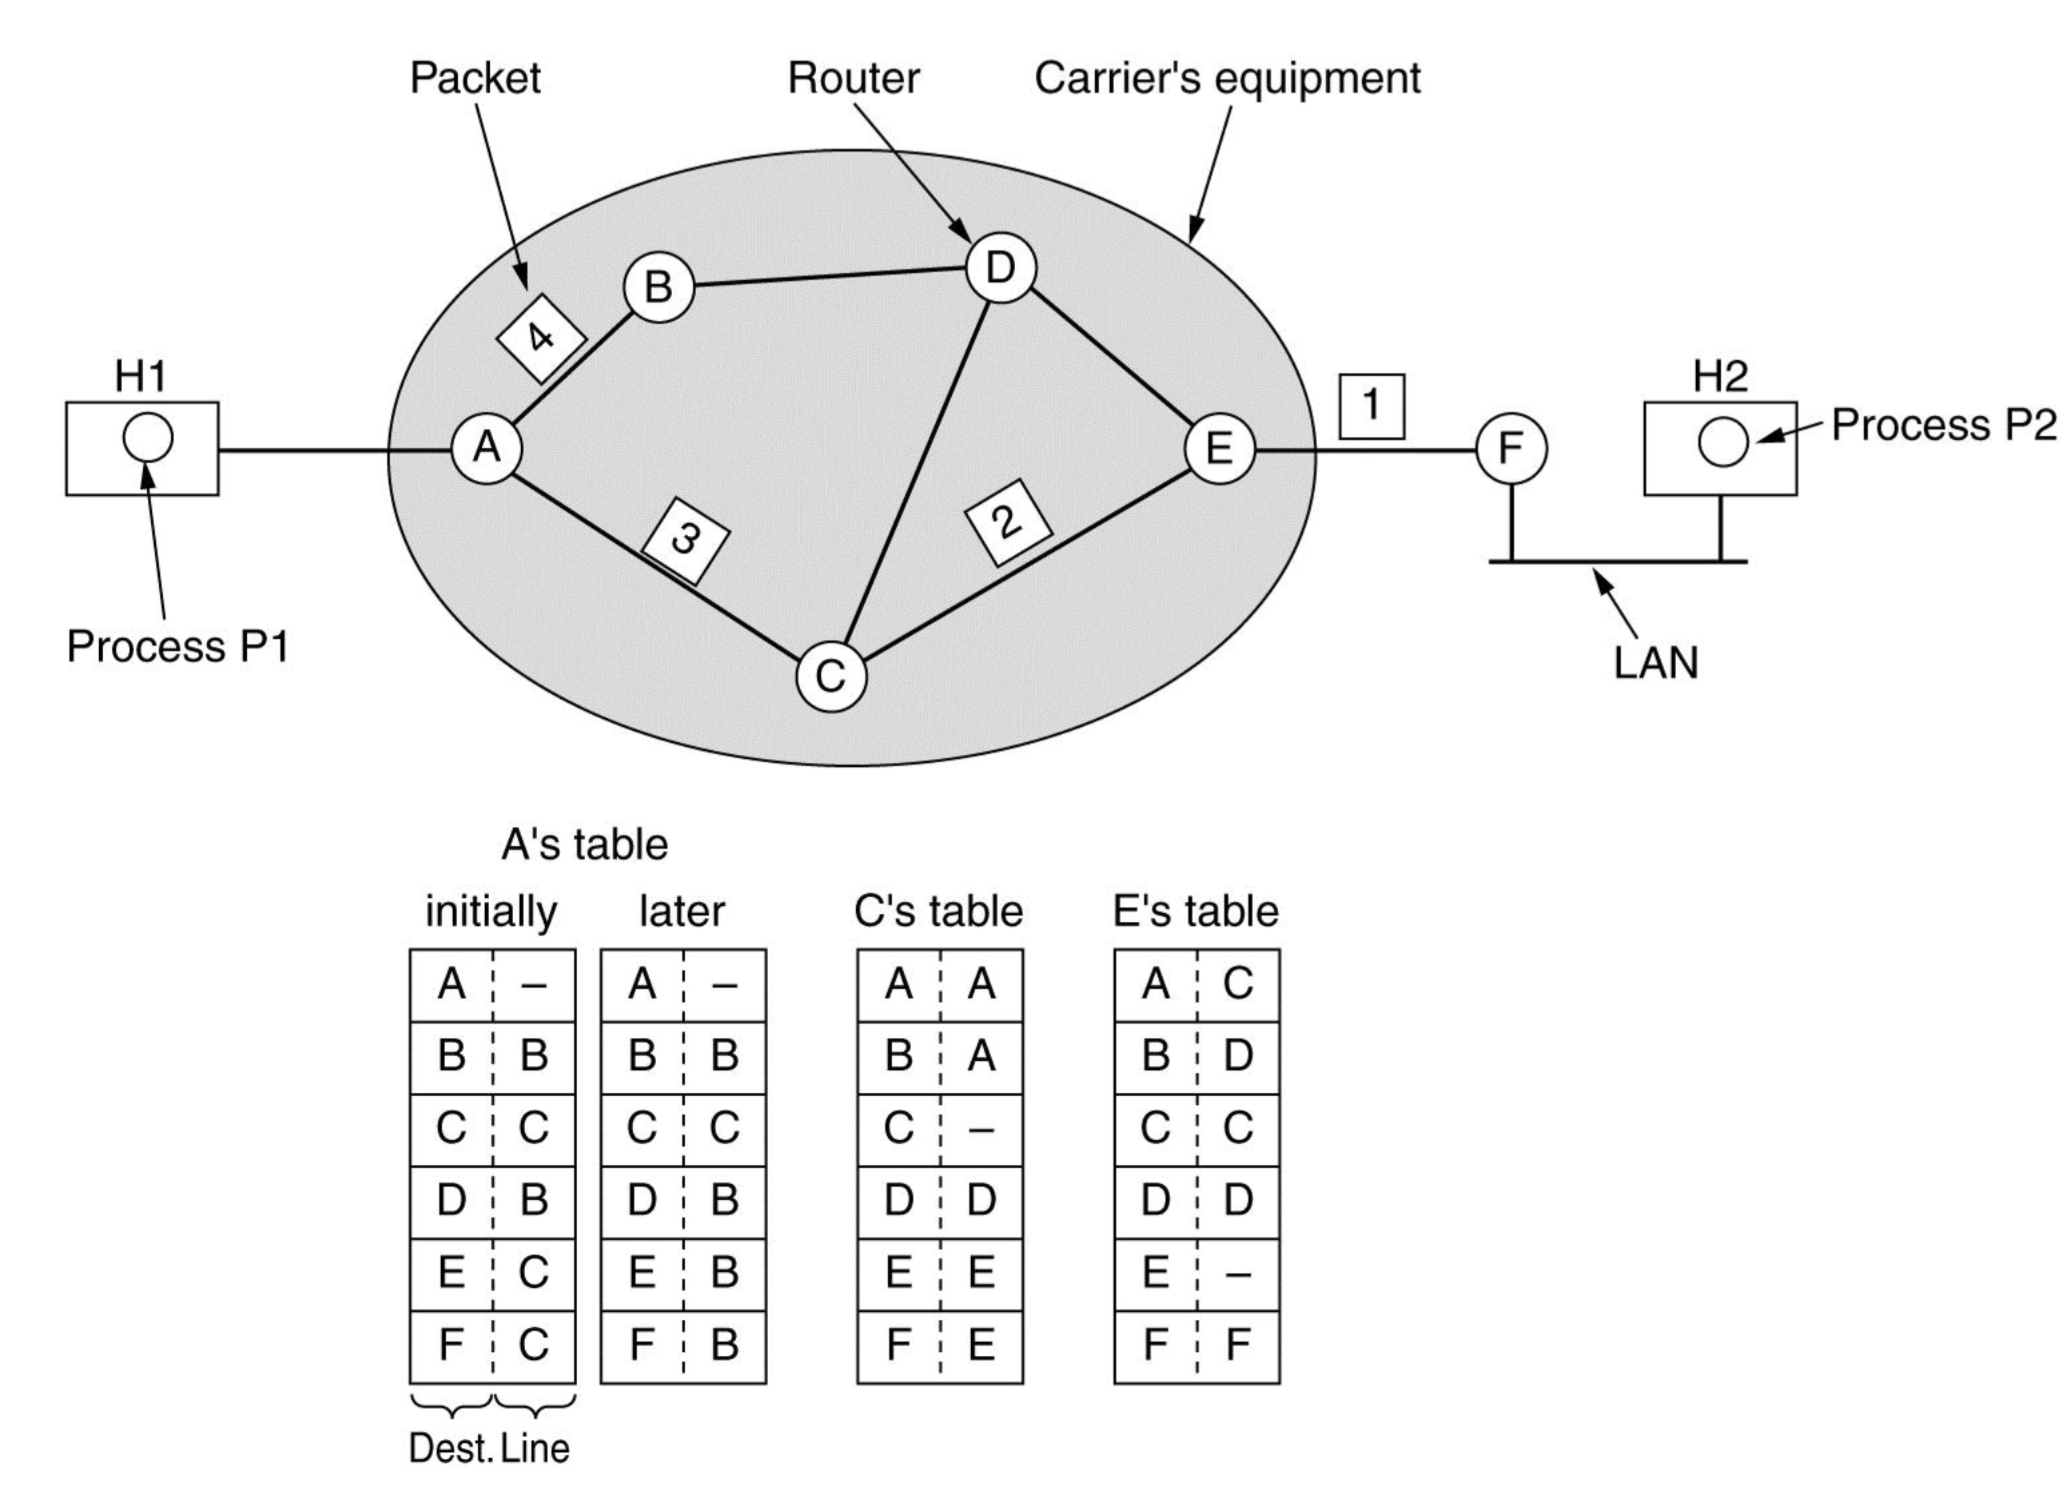
\includegraphics[width=8cm, height=6cm]{./imagenes/norientado.png} 
\end{center}

\par Problema:  
\par IP es el ejemplo dominante de un servicio de red sin conexión. Cada paquete 
transporta una dirección IP de destino que los enrutadores usan para reenviar cada 
paquete por separado. Las direcciones son de 32 bits en los paquetes IPv4 y de 128 
bits en los paquetes IPv6.

\subsection{Implementación del servicio orientado a conexión}
	\begin{itemize}\itemsep=0pt
			\item \textbf{Conexiónes o circuitos virtuales (CV)}
			\item \textbf{Subred de Circuitos Virtuales} = subred
			\item Evitar la necesidad de elegir una nueva ruta para cada paquete enviado. 
			La ruta de una conexión se almacena en tablas en los enrutadores, esta ruta se 
			usa para todo el tráfico que fluye a través de la conexión.
			\item Cada paquete lleva un identificador de CV.
			\item Liberación de conexión: se termina el CV
			\item Se paga el precios del espacio de tabla en los enrutadores. El uso de CVs 
			requiere una fase de configuración que consume tiempo y recursos.
	\end{itemize}

\begin{center} 
	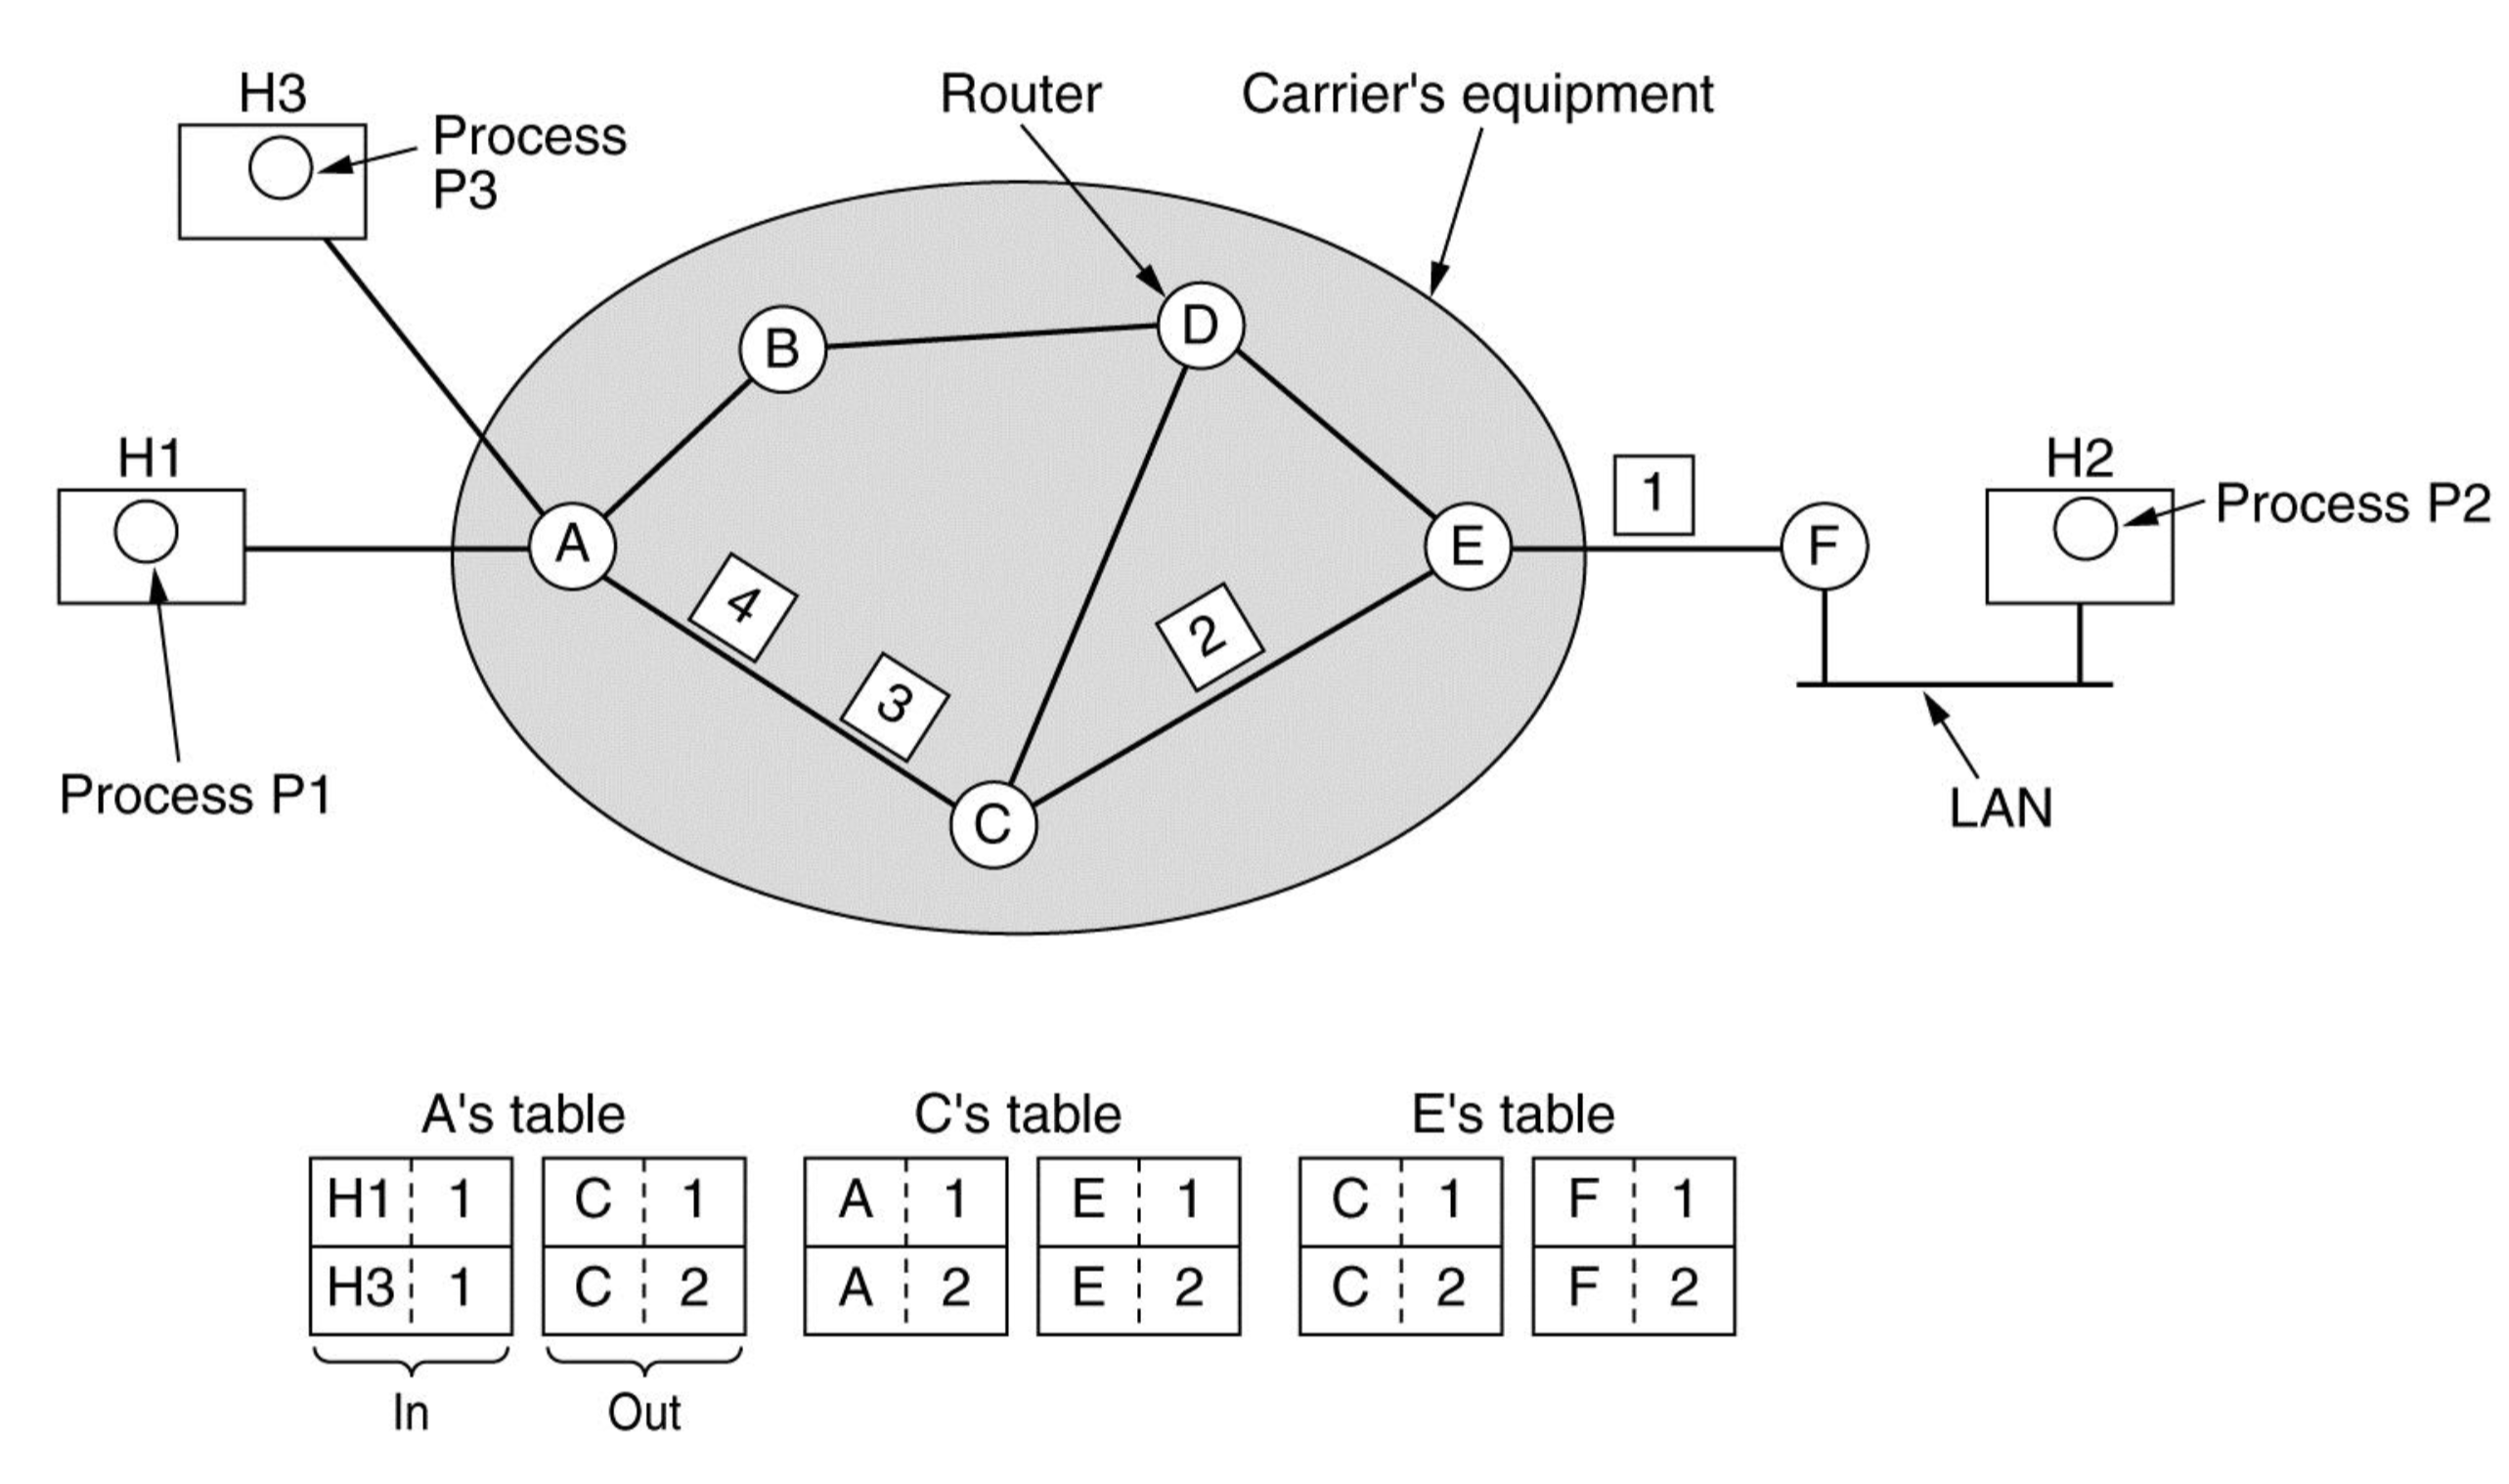
\includegraphics[width=8cm, height=6cm]{./imagenes/orientado.png} 
\end{center}

\par En algunos contextos, a este proceso se le conoce como conmutación mediante 
etiquetas. MPLS (MultiProtocol Label Swithching) es un ejemplo de servicio de red 
orientado a conexión. Se utiliza dentro de las redes de ISP en Internet, en donde los 
paquetes IP se envuelven en un encabezado MPLS que tiene un identificador de 
conexión o etiqueta de 20 bits.
	
\subsection{Comparación entre las redes de circuitos virtuales y las redes de datagramas}
	Dentro de la red existen ventajas y desventajas entre los circuitos virtuales y los 
	datagramas. Una de ellas tiene que ver con el tiempo de configuración y el tiempo de 
	análisis de la dirección. El uso de circuitos virtuales requiere una fase de 
	configuración que necesita tiempo y recursos. Sin embargo, una vez que se paga 
	este precio, es fácil averiguar qué hacer con un paquete de datos en una red de 
	circuitos virtuales: el enrutador sólo usa el número de circuito para buscar en una 
	tabla y encontrar hacia donde va el paquete. En una red de datagramas no se 
	requiere configuración, pero se requiere un procedimiento más complicado para 
	localizar la entrada correspondiente al destino.

	\begin{center} 
		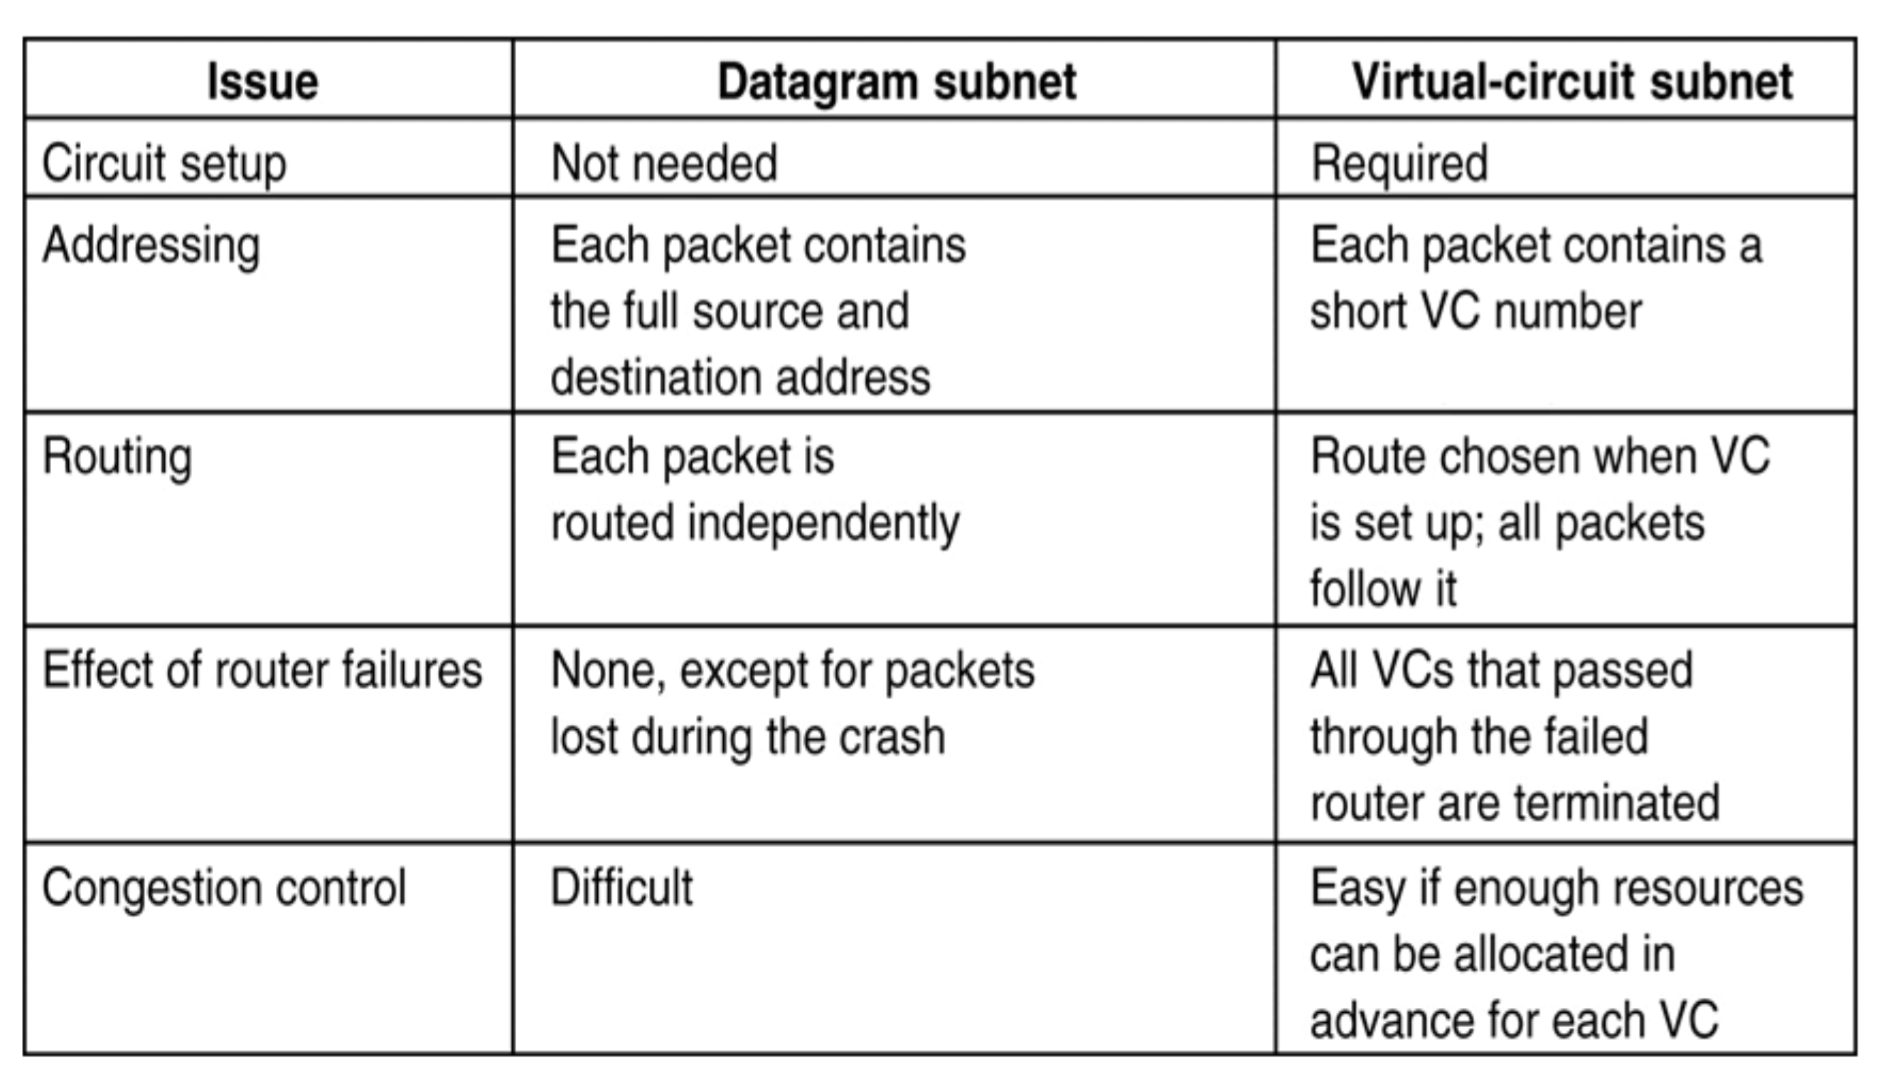
\includegraphics[width=10cm, height=6cm]{./imagenes/comparacion.png}
	\end{center}
	
	\begin{itemize}
		\item Si se cae un enrutador en CV: se pierde su memoria, y todos los CV que 
		pasan por el tendrán que abortarse.
		\item Si se cae un enrutador de datagramas: solo sufrirán los usuarios cuyos 
		paquetes estaban encolados en el enrutador en el momento de la falla, 
		dependiendo de si había confirmado o no su recepción, tal vez ni siquiera todos 
		ellos.
	\end{itemize}


\section{Algoritmos de enrutamiento}
	\par El algoritmo de enrutamiento es aquella parte del software de la capa de red 
	responsable de decidir por cuál línea de salida transmitirá un paquete entrante. Si la 
	red usa datagramas de manera interna, esta decisión debe tomarse cada vez que 
	llega un paquete de datos, dado que la mejor ruta podría haber cambiado desde la 
	última vez. Si la red usa circuitos virtuales internamente, las decisiones de 
	enrutamiento se toman sólo al establecer un circuito virtual nuevo. En lo sucesivo, 
	los paquetes de datos simplemente siguen la ruta ya establecida. Este último caso a 
	veces se llama enrutamiento de sesión, dado que una ruta permanece vigente 
	durante toda una sesión.
	\par En ocasiones es útil distinguir entre el enrutamiento, que es el proceso que 
	consiste en tomar la decisión de cuáles rutas utilizar, y el reenvío, que consiste en la 
	acción que se toma cuando llega un paquete. Podemos considerar que un enrutador 
	tiene dos procesos internos. Uno de ellos maneja cada paquete conforme llega, y 
	después busca en las tablas de enrutamiento la línea de salida por la cual se enviará. 
	Este proceso se conoce como reenvío. El otro proceso es responsable de llenar y 
	actualizar las tablas de enrutamiento. Es ahí donde entra en acción el algoritmo de 
	enrutamiento.
	
	\par Propiedades que todo algoritmo de enrutamiento debe poseer:
		\begin{itemize}
			\item \textbf{Robustez:} una vez que una red entra en operación, deberá
			funcionar 			
			continuamente durante años. Durante ese período habrá fallas de hardware y de 
			software de todo tipo. Los hosts, enrutadores y líneas fallarán en forma 
			repetida y la topología cambiará muchas veces.
			\par El algoritmo de enrutamiento debe ser capaz de manejar los cambios de 
			topología y tráfico sin requerir que aborten todas las actividades en todos los 
			hosts y el reinicio de la red con cada caída de un enrutador.
			\item \textbf{Optimización:} por un lado se intenta minimizar el 
			retardo medio de los paquetes, por otro aumentar al máximo la velocidad real 
			de transporte en la red. 
			\par Estas dos metas están en conflicto. Como término medio muchas redes 
			intentan minimizar el número de saltos que tiene que dar un paquete.
			La reducción de la cantidad de saltos reduce el retardo y también el consumo 
			de ancho de banda, lo que a su vez mejora la velocidad real de transporte.
			\item \textbf{Equidad:} implica que todos los hosts deben poder usar la subred 
			ya sea para enviar o para recibir.
			\par La equidad y la optimización son con frecuencia metas contradictorias. Por 
			ende se requiere de un punto medio entre la eficiencia global y la equidad hacia 
			las conexiones individuales.
			\item \textbf{Sencillez:} apenas requiere comentarios. Es algo que todos los 
			algoritmos de enrutamiento deberían tener. 
			\item \textbf{Estabilidad:} también es una meta importante para el algoritmo 
			de enrutamiento. Existen algoritmos de enrutamiento que nunca convergen 
			hacia un conjunto de rutas fijo, sin importar el tiempo que permanezcan en 
			operación. Un algoritmo estable alcanza el equilibrio y lo conserva. Además 
			debe converger con rapidez, ya que se puede interrumpir la comunicación hasta 
			que el algoritmo de enrutamiento haya llegado a un equilibrio.
		\end{itemize}
		
		\par Los algoritmos de enrutamiento pueden agruparse en dos clases: 
		\begin{enumerate}
		
			\item  \textbf{\emph{Los algoritmos no adaptativos: }} no basan sus 
			decisiones de enrutamiento en mediciones o estimaciones del tráfico y la 
			topología actuales.
			\begin{itemize}
				\item La decisión de qué ruta se usará para ir de I a J se toma por 
				adelantado.
				\item A esto se lo conoce como enrutamiento estático.
				\item Ejemplos: enrutamiento de caminos más cortos, inundación.
			\end{itemize}
			
			\item \textbf{\emph{Los algortimos adaptativos:}} cambian sus decisiones de 
			enrutamiento para reflejar los cambios de topología, y por lo general también 
			del tráfico.
			\par Los algoritmos adaptivos difieren en:
			\begin{itemize}
				\item El lugar donde obtienen su información, localmente en los enrutadores 
				adyacentes o en todos los enrutadores.
				\item El momento de cambio de sus rutas (i.e. de sus tablas de 
				enrutamiento). Hay varias opciones, ellas son: cada cierta cantidad de 
				segundos, cuando cambia la carga, o cuando cambia la topología.
				\item La métrica usada para la optimización: distancia, número de saltos, 
				tiempo estimado de tránsito, etc.
			\end{itemize}
			\par Ejemplos: enrutamiento de vector de distancia, enrutamiento de estado de 
			enlace.		
		\end{enumerate}

\subsection{Principio de optimización}
	\par Establece que si un enrutador \textit{J} está en ruta óptima 
	del enrutador \textit{I} al enrutador \textit{K}, entonces la ruta óptima de \textit{J}
	a \textit{K} también está en la misma ruta.
	\par Como consecuencia directa del principio de optimización, podemos ver que el 
	grupo de rutas óptimas de todos los orígenes a un destino dado forman un árbol con 
	raíz en el destino. Dicho árbol se conoce como \textit{árbol sumidero} y se ilustra en 
	la figura, donde la métrica de distancia es el número de saltos. El objetivo de todos 
	los algoritmos de enrutamiento es descubrir y usar los árboles sumidero para todos 
	los enrutadores.
	
	\begin{center}
		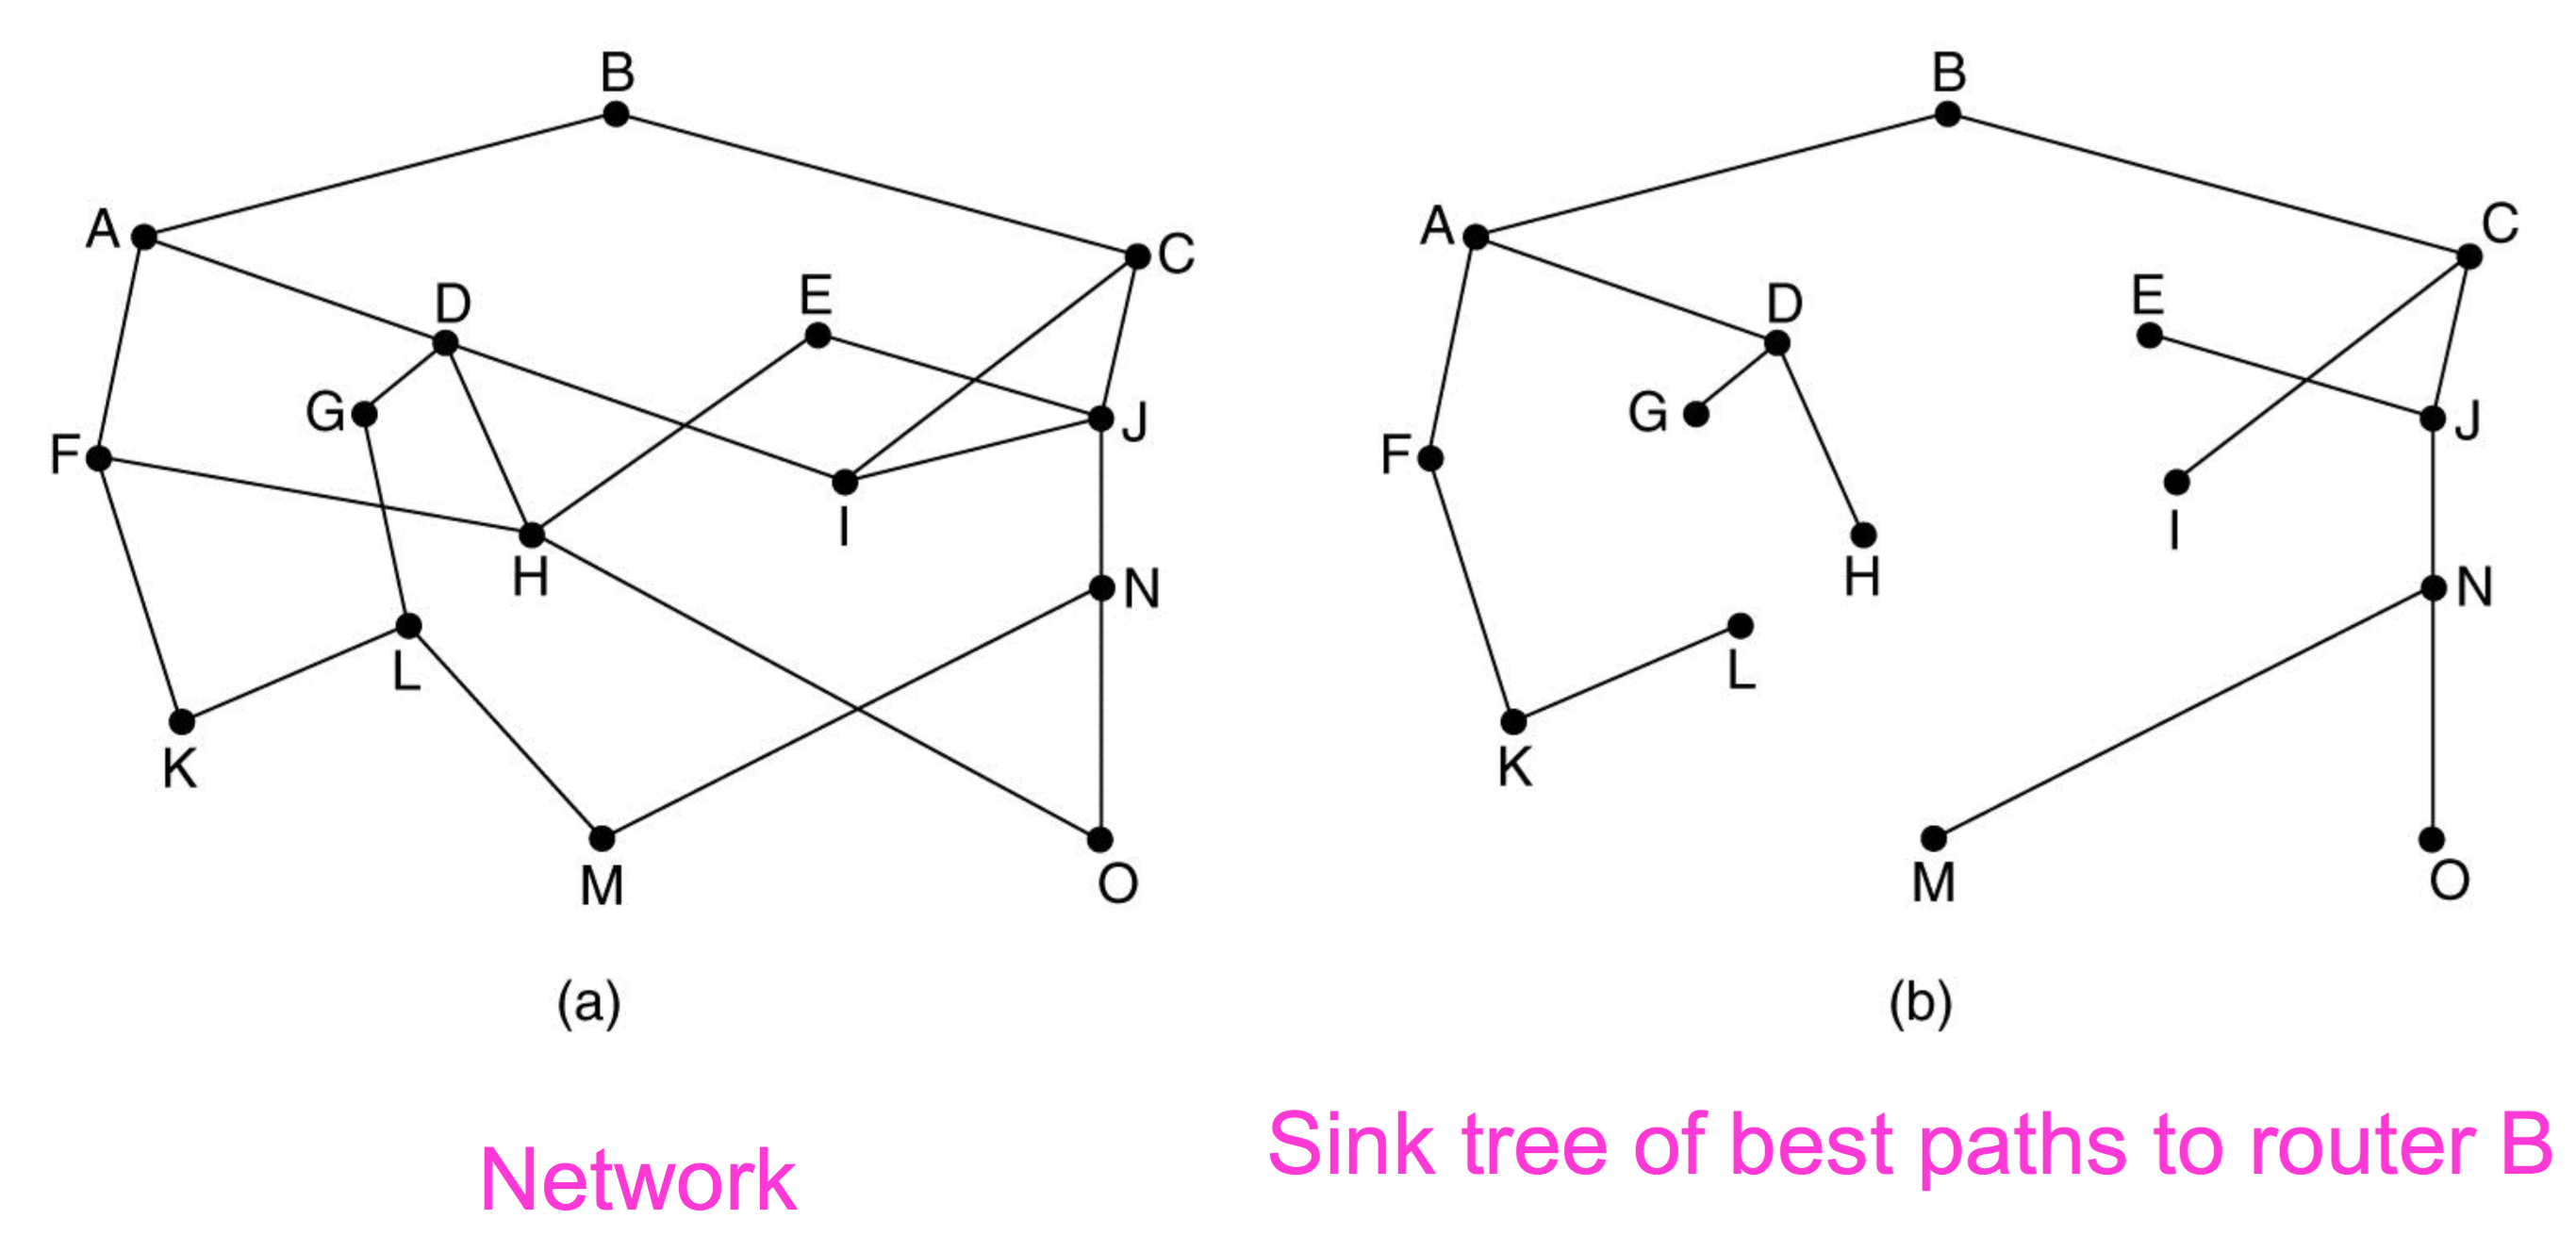
\includegraphics[width=10cm, height=6cm]{./imagenes/optimalidad.png}
	\end{center}

	\par Por ende la meta de todos los algoritmos de enrutamiento es descubrir y utilizar 
	los árboles sumideros de todos los enrutadores.
	
	\par Comenzaremos estudiando algoritmos estáticos, los mismos no son muy 
	buenos, pero veremos que pequeñas variantes de ellos son usados por los algoritmos 
	adaptivos.

\subsection{Algoritmo de la ruta más corta}
	\par La idea es construir un grafo de la red, en donde cada nodo del grafo 
	representa un enrutador y cada arco del grafo representa una línea o enlace de 
	comunicaciones. Para elegir una ruta entre un par específico de enrutadores, el 
	algoritmo simplemente encuentra la ruta más corta entre ellos en el grafo.

	\par Una manera de medir la longitud de una ruta es mediante el número de saltos. 
	Otra métrica es la distancia geográfica en kilómetros, etc. En el caso más general, las 
	etiquetas de los arcos podrían calcularse como función de la distancia, ancho de 
	banda, tráfico medio, costo de comunicación, longitud media de las colas, retardo 
	medio, y otros factores.

	\par Se conocen varios algoritmos para calcular la ruta más corta entre dos nodos de 
	un grafo. Uno de éstos se debe a Dijkstra.


	\par \textbf{Algoritmo de Dijktra:}
		\begin{itemize}
			\item Calculamos la ruta más corta posible entre \emph{s} y \emph{t}
			comenzando por el nodo de destino \emph{t}.
			\item El algoritmo calcula un árbol sumidero en la subred.
			\item Cada nodo se etiqueta con su distancia al nodo de origen a través de la 	
			mejor ruta conocida (al comienzo todos los nodos tienen etiqueta <). Mientras 
			avanza el algoritmo las etiquetas pueden cambiar reflejando mejores rutas.
 			\item Una etiqueta puede ser tentativa o permanente. Inicialmente todas las 
 			etiquetas son tentativas. Cuando se descubre que una etiqueta representa la 
 			ruta más corta del origen a ese nodo, se vuelve permanente y no cambia más.
			\item Se tiene una iteración para la cua lsiempre hay un nodo de trabajo. Ese 
			nodo de trabajo es el nodo tentativo con la menor etiqueta calculado en el paso 
			de iteración anterior (Inicialmente el nodo de trabajo es \emph{t}).
			
			En cada paso de la iteración se actualizan las etiquetas de los nodos tentativos 
			siempre y cuando el nodo de trabajo ayude a encontrar una ruta mejor.
		\end{itemize}

	\begin{center}
	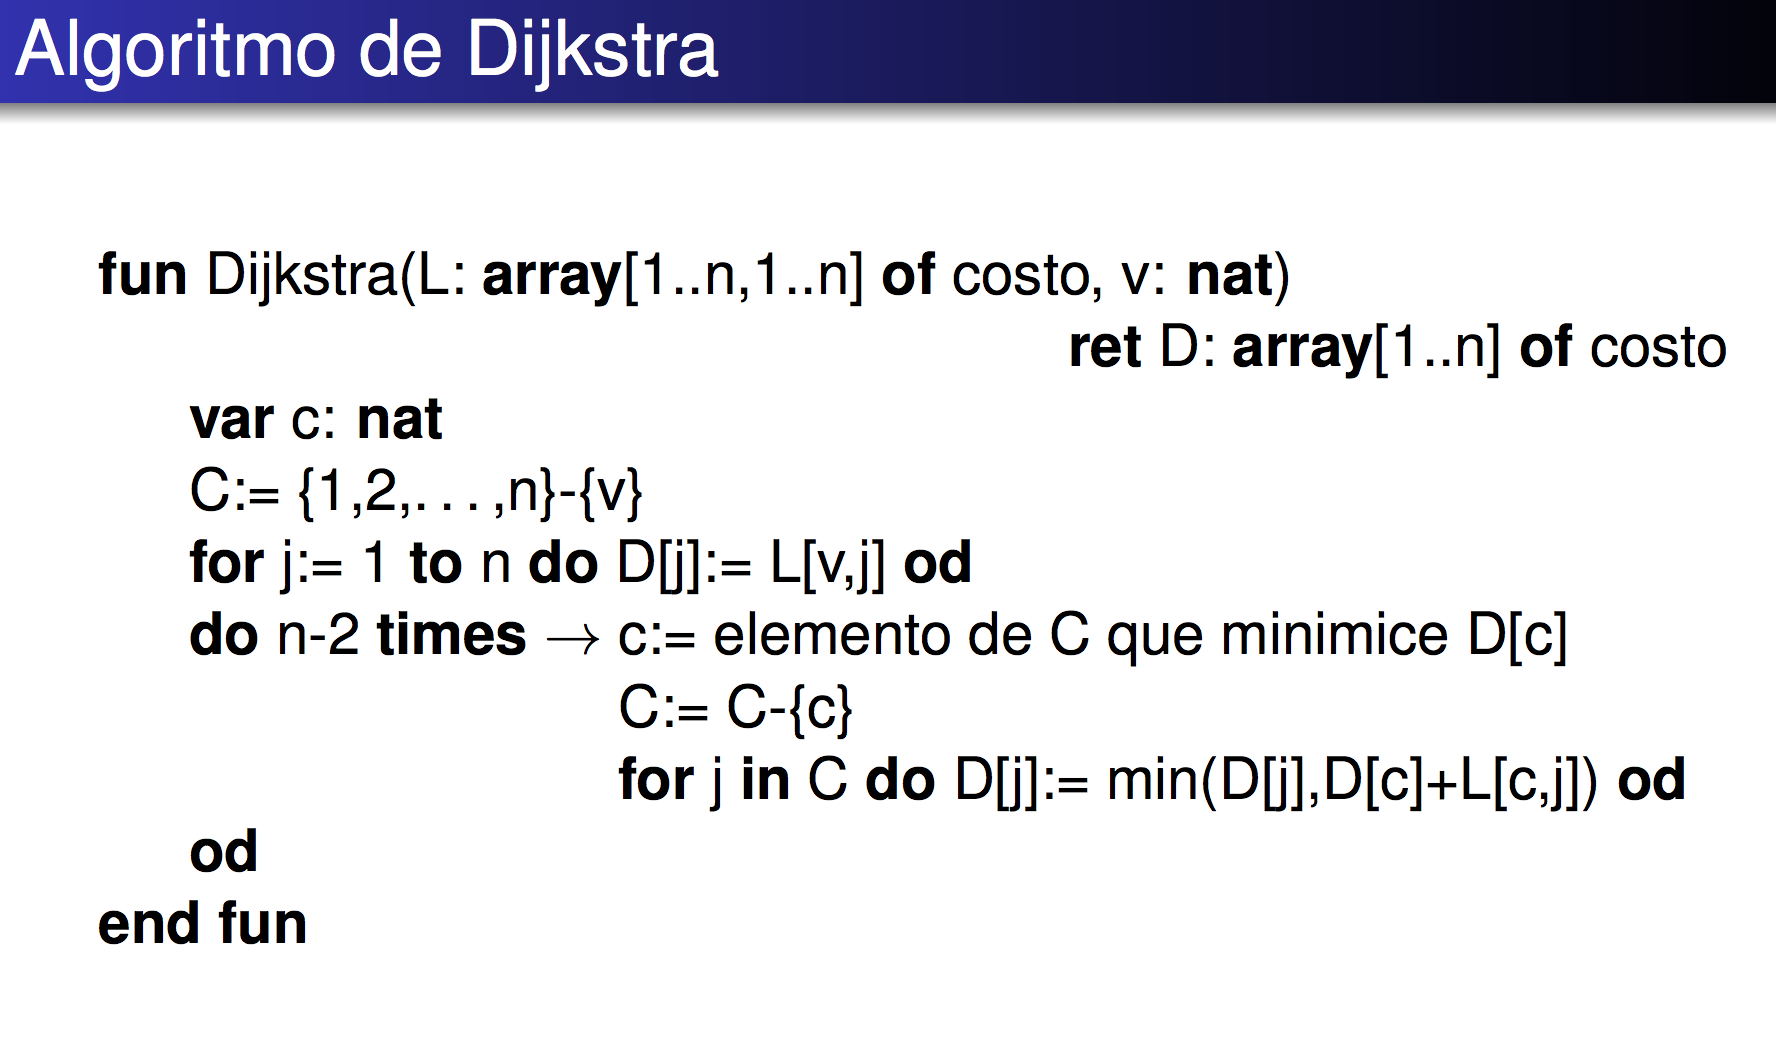
\includegraphics[width=8cm, height=5cm]{./imagenes/dijktra.png} 

	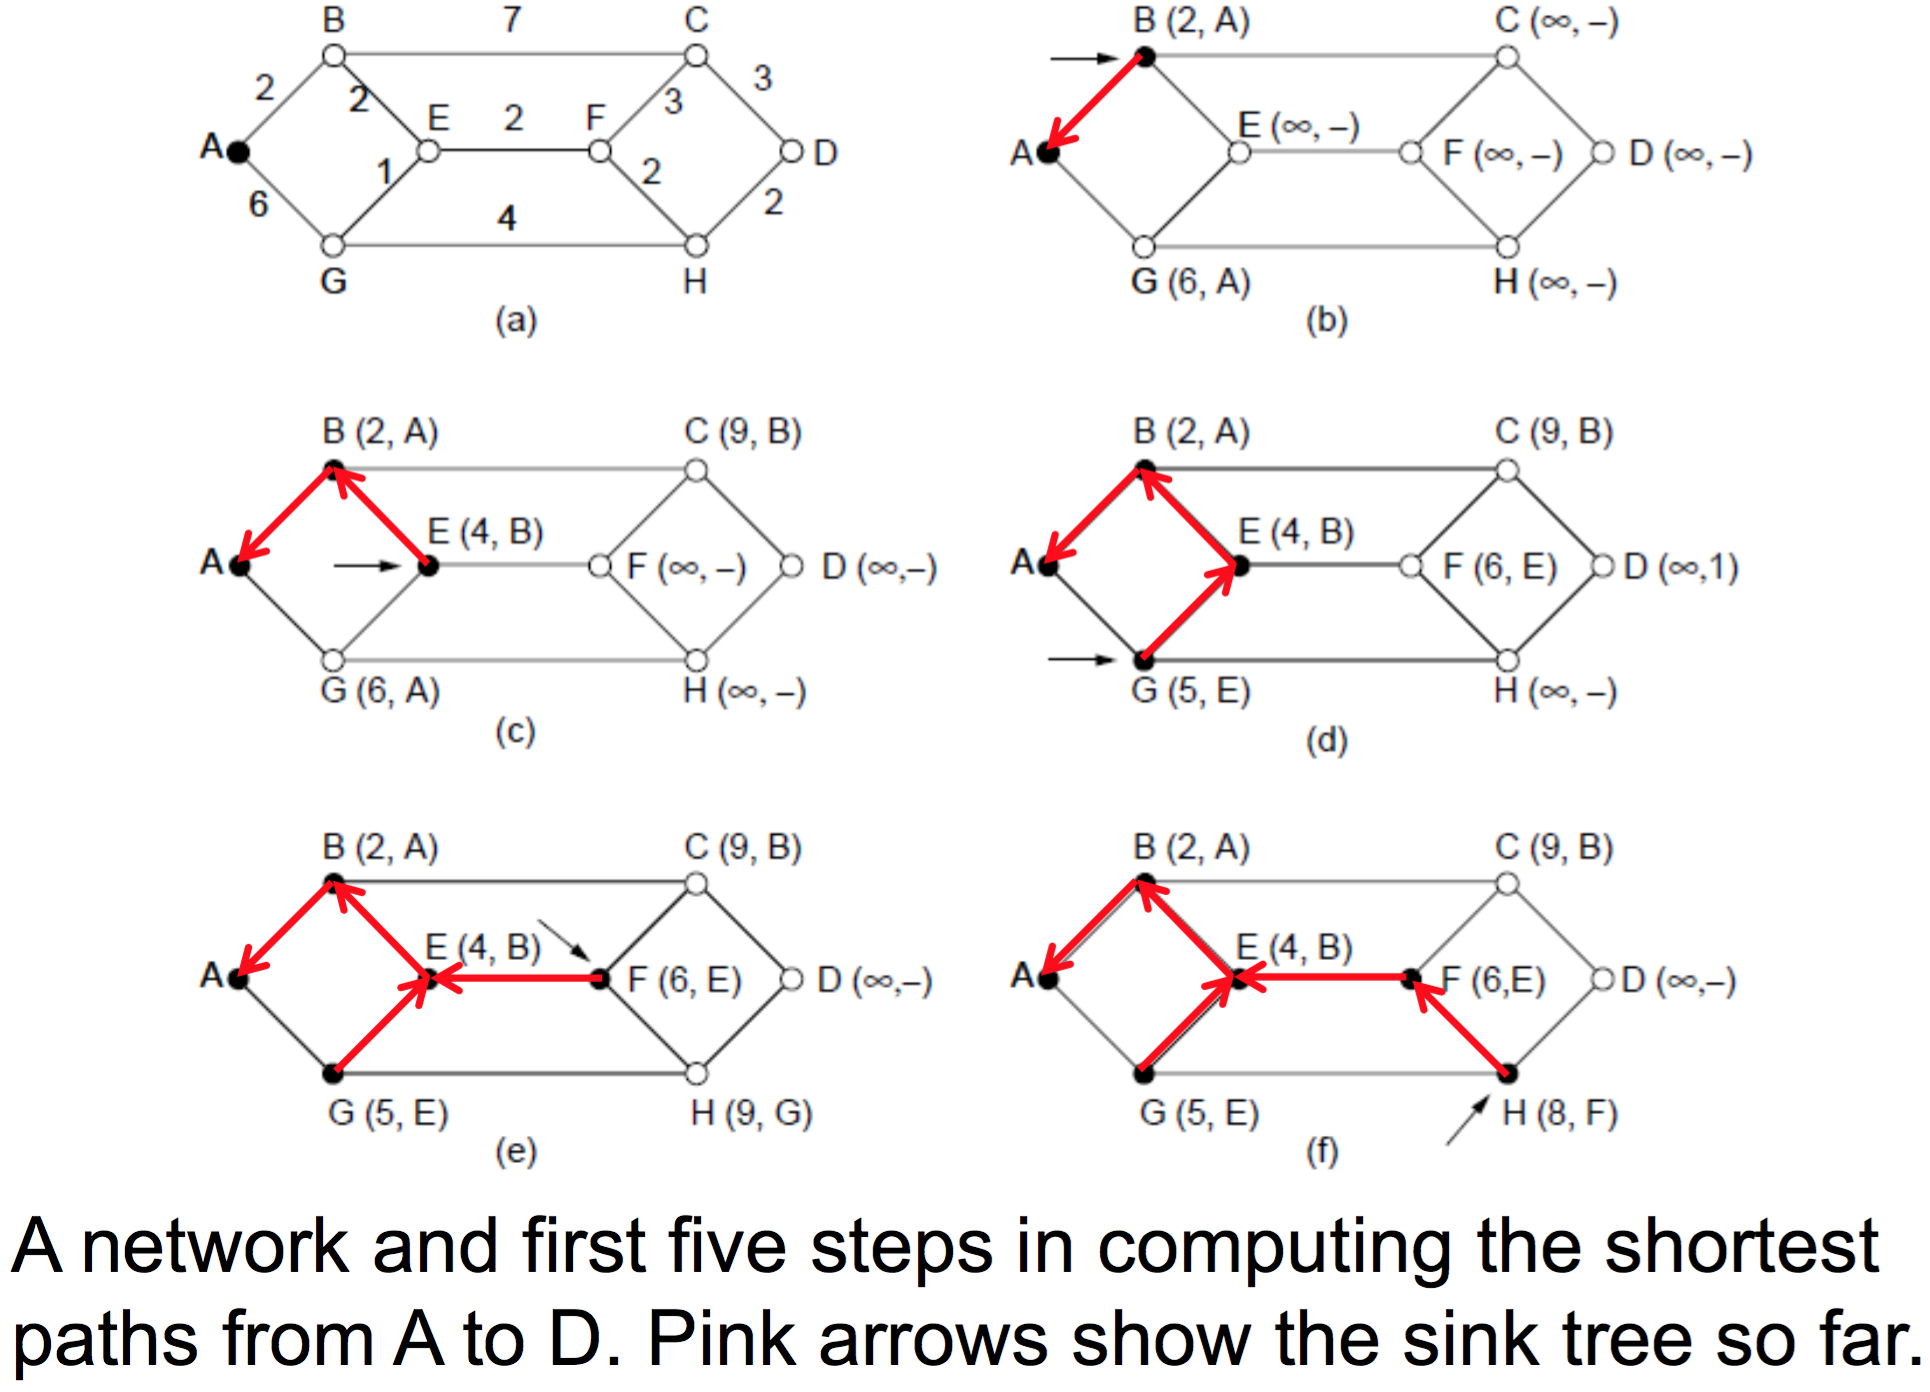
\includegraphics[width=10cm, height=6cm]{./imagenes/caminos.png}
	\end{center}

\subsection{Inundación}
	\par Otro algoritmo estático es la inundación, en la que cada paquete de entrada se 
	envía por cada una de las líneas de salida, excepto aquella por la que llegó.
    Esta idea tiene un problema, la inundación genera grandes cantidades de paquetes 
    duplicados; a menos que se tomen algunas medidas para limitar el proceso. Veamos 
    algos de estas ideas:

	\begin{itemize}
		\item Solución 1: integrar un contador de saltos en el encabezado de cada 
		paquete, que disminuya con cada salto y el paquete se descarte cuando el 
		contador llega a 0. Lo ideal es inicializar el contador de saltos a la longitud de la 
		ruta entre el origen y el destino. Si el emisor desconoce el tamaño de la ruta, 
		puede inicializar el contador al peor caso, es decir, al diámetro total de la subred.
		
		\item Solución 2: llevar un registro de los paquetes difundidos para evitar 
		enviarlos por segunda vez. Hacer que el enrutador de origen ponga un número de 
		secuencia en cada paquete que recibe de sus hosts. Para cada enrutador de origen 
		hay una lista con los números de secuencia originados en ese enrutador que ya ha 
		visto. Si un paquete de entrada está en la lista, no se difunde.

		Para evitar que las listas crezcan sin límites podemos agregar una columna 
		contador que indica el mayor número de secuencia tal que llegaron paquetes con 
		todos los numeros de secuencia anteriores desde ese enrutador de origen.
		
		\item Solución 3: Una variación de la inundación, un poco mas práctica, es la 
		inundación selectiva. Los enrutadores no envían cada paquete de entrada por 
		todas las líneas, sino solo por aquellas que van aproximadamente en la dirección 
		correcta.

		A nivel de información, se necesita saber en qué  dirección va cada línea y en qué 
		dirección está el destino.
		
		\par La inundación no es práctica en la mayoría de las aplicaciones, pero tiene
		algunos usos, por ejemplo, en aplicaciones militares, en aplicaciones distribuidas 
		de bases de datos. La inundación siempre elige la ruta más corta posible porque 
		escoge en paralelo todas las rutas posibles. En consecuencia ningún otro 
		algoritmo puede producir un retardo más corto (si ignoramos la sobrecarga 
		generada por el proceso de inundación mismo).
		
	\end{itemize}
		
\subsection{Enrutamiento por vector de distancia}

	\par 	Existen dos algoritmos dinámicos que son los más populares: el enrutamiento 
	por vector de distancia y el enrutamiento por estado del enlace. En esta sección 
	veremos el primer algoritmo, en la siguiente estudiaremos el segundo.
	\par En el enrutamiento por vector de distancia, cada enrutador mantiene una tabla 
	de enrutamiento indizada por cada enrutador de la red. Esta entrada consta de dos 
	partes:
	\begin{itemize}
			\item La línea preferida de salida a usar para ese destino
			\item Una estimación del tiempo o distancia a ese destino. 
	\end{itemize}
	\par La distancia se podría medir como la cantidad de saltos, o se podría usar otra 
	métrica, como vimos al calcular las rutas más cortas. 
	\par 	Estas tablas se actualizan intercambiando información con los vecinos. Este 
	algoritmo se usó en Internet con el nombre \textbf{RIP}.
	
	\par Se supone que el enrutador conoce la “distancia” a cada uno de sus vecinos.
		\begin{itemize}
			\item Si la métrica es de saltos, la distancia es un salto.
			\item Si la métrica es la longitud de la cola, el enrutador simplemente examina 
			cada cola.
			\item Si la métrica es el retardo, el enrutador puede medirlo con paquetes de 
			ECO que el receptor simplemente marca con la hora y los regresa tan rápido 
			como puede.
		\end{itemize}
	\par Suponga que el retardo se usa como métrica y que el enrutador conoce el 
	retardo a cada uno de sus vecinos. Una vez cada \textit{T} mseg, cada enrutador 
	envía a todos sus vecinos una lista de sus retardos estimados a cada destino.
	También recibe una lista similar de cada vecino. Imagine que la tabla
	\textit{$T_{x}$} acaba de llegar del vecino \textit{X}, en donde \textit{$X_{i}$} es 
	la 	estimación respecto al tiempo que le toma llegar al enrutador \textit{i}. Si el 	
	enrutador sabe que 	el retardo a 	\textit{X} es de \textit{$m_{x}$} mseg, también 
	sabe que puede llegar al enrutador \textit{i} a través de \textit{X} en 
	\textit{$X_{i}$} $+$ \textit{$m_{i}$} mseg. Al efectuar este cálculo para cada 
	vecino, un enrutador puede encontrar la estimación que parezca ser la mejor y usar 
	esa estimación, así como el enlace correspondiente, en su \textbf{nueva tabla de 
	enrutamiento}. Cabe mencionar que en este cálculo no se utiliza la antigua tabla de 
	enrutamiento.

	\par El enrutamiento por vector reacciona con rapidez a las buenas noticias, pero 
	con lentitud ante las malas. Considere un enrutador cuya mejor ruta al destino 
	\textit{X} es larga. Si en el siguiente intercambio el vecino \textit{A} informa 
	repentinamente un retardo corto a \textit{X}, el enrutador simplemente se conmuta 
	a modo de usar la línea a A para enviar tráfico hasta X.
Supongamos que la métrica de retardo es el numero de saltos.
 Las buenas noticias se difunden a razón de un salto por intercambio.
 En una subred cuya ruta mayor tiene una longitud de N saltos, en un lapso de N intercambios todo el mundo sabrá sobre las líneas y enrutadores recientemente revividos.
La razón de porque las malas noticias viajan con lentitud es: ningún enrutador jamás tiene un valor mayor en más de una unidad que el mínimo de todos sus vecinos.
Gradualmente todos los enrutadores elevan cuentas hacia el infinito, pero el número de intercambios requeridos depende del valor numérico usado para el infinito.
Si la métrica usada es el número de saltos, es prudente hacer que el infinito sea igual a la ruta más larga más 1.

Si la métrica es el retardo de tiempo no hay un límite superior
bien definido,
se necesita un valor alto para evitar que una ruta con un retardo grande sea tratada como si estuviera desactivada.
Este es el problema de la cuenta hasta el infinito.
Se han hecho varios intentos para resolverlo, pero ninguno funciona bien
en general.
La esencia del problema consiste en que cuando X indica Xi a E, E no tiene forma de saber si el destino i está en alguna ruta en funcionamiento.

\subsection{Enrutamiento por estado del enlace}
	\par La idea detrás del enrutamiento por estado del enlace es bastante simple y 
	se puede enunciar en cinco partes. Cada enrutador debe realizar lo siguiente para 
	hacerlo funcionar:

	\begin{enumerate}
		\item Descubrir a sus vecinos y conocer sus direcciones de red: esto lo realiza 
		enviando un paquete HELLO especial a cada línea punto a punto. Se espera que 
		el 	enrutador del otro extremo regrese una respuesta indicando quién es. Estos
		nombres deben ser globalmente únicos.

		\item Establecer la métrica de distancia o de costo para cada uno de sus vecinos:
		el AEEE requiere que cada enrutador tenga una idea razonable del retardo a cada 
		uno de sus vecinos. Una forma de determinarlo es enviar un paquete ECHO 
		especial a través de la línea, una vez que llegue al otro extremo, éste debe 
		regresarlo inmediatamente.

		\par Si se mide el tiempo de ida y vuelta y se divide por $2$, el enrutador emisor 
		puede tener una idea razonable del retardo. Pero esto tiene un problema, ya que 
		el algoritmo asume de manera implícita que los retardos son simétricos, lo cual no 
		siempre es el caso.

		\par Un aspecto importante es si se debe tener en cuenta la carga al medir el 
		retardo. Para considerar la carga, el temporizador debe iniciarse cuando el paquete 
		ECHO se ponga en la cola. Para ignorar la carga, el temporizador debe iniciarse 
		cuando el paquete ECHO alcance el frente de la cola.
		
		\par Cuando un enrutador puede escoger entre dos líneas con el mismo ancho de 
		banda, una con carga alta continua y otra sin ella, considerará como ruta más 
		corta la de la línea sin carga. Esta selección resultará en un mejor desempeño. 		
		Desgraciadamente también hay un argumento en contra de la inclusión de la carga 
		en el cálculo del retardo.

		\item Construir un paquete que indique todo lo que acaba de aprender: Cada 
		enrutador construye un paquete des estado de enlace (LSP) que contiene todos 
		los datos:
		\begin{itemize}
			\item Identidad del emisor
			\item Numero de secuencia
			\item Edad
			\item Lista de (vecino, retardo al vecino)
		\end{itemize}

		\par los paquetes deben ser construirlos de manera periódica, es decir, a 
		intervalos regulares o cuando ocurra un evento significativo, como la caída o la 
		reactivación de la línea o de un vecino, o el cambio apreciable de sus propiedades.

		\item Enviar este paquete a todos los demás enrutadores y recibir paquetes de 		
		ellos: la parte más complicada del algoritmo es la distribución confiable de los 
		paquetes de estado del enlace.
		
		\par La idea fundamental es usar inundación para distribuir los paquetes de 
		estado 
		del enlace, llevando un registro de los paquetes difundidos. A fin de mantener 
		controlada la inundación, cada paquete contiene un número de secuencia que se 
		incrementa con cada paquete nuevo enviado (desde su enrutador de origen).
		\par Los enrutadores llevan el registro de todos los pares (enrutador de origen, 
		secuencia) que ven. Para cada enrutador de origen el paquete recibido con 
		número de secuencia más grande es el que importa, los anteriores no.

		\item Calcular la ruta más corta a todos los demás enrutadores.
	\end{enumerate}

	

\subsection{Enrutamiento jerárquico}
\subsection{Enrutamiento por difusión}
\section{Algoritmos de control de congestión}
\subsection{Métodos para el control de la congestión}
\subsection{Enrutamiento consciente del tráfico}
\subsection{Control de admisión}
\subsection{Regulación del tráfico}
\subsection{Desprendimiento de carga}

\section{La capa de internet}
\subsection{El protocolo IP versión 4}
\subsection{Direcciónes IP}
\subsection{IP versión 6}
\subsection{Protocolos de control de Internet}
\subsection{Conmutación mediante etiquetas y MPLS}
\subsection{OSPF: un protocolo de enrutamiento de puerta de enlace interior}

\subsection{BGP: el protocolo de enrutamiento de Puerta de Enlace Exterior}
	\par Los enrutadores de protocolo de puerta de enlace exterior tienen que 
	preocuparse en gran parte por la política. Muchas veces se quiere mantener las 
	políticas privadas; porque los Sistemas Autónomos (SA) compiten entre sí (ej: PSI 
	competidores).	
	\par Las políticas típicas implican consideraciones políticas, de seguridad, o 
	económicas. Algunos ejemplos de posibles restricciones de enrutamiento son:
		\begin{enumerate}
			\item  No transportar tráfico comercial en la red educativa.
			\item Nunca enviar tráfico del Pentágono por una ruta a través de Irak.
			\item Usar TeliaSonera en vez de Verizon porque es más económico.
			\item No usar AT and T en Australia porque el desempeño es pobre.
			\item El tráfico que empieza o termina en Apple no debe transitar por Google.
		\end{enumerate}

	\par Para enrutamiento inter SA encontrar un camino óptimo es prácticamente 
	imposible. Cada SA corre su propio protocolo interno y usa cualquier esquema para 
	asignar métricas a los caminos. Es imposible calcular costos de caminos 
	significativos para caminos que cruzan varios SA.
	\par Enrutamiento inter SA solo avisa alcanzabilidad, por lo tanto, a lo más puedo 
	tener caminos de SA para ir de un origen a un destino.
	
	\par Para el enrutamiento es necesario encontrar algún camino de SA para el destino 
	deseado que es libre de ciclos. Además los caminos deben respetar las políticas de 
	los SA a lo largo del camino. Donde una política significan reglas que se refieren a 
	preferencias de enrutamiento y a limitaciones de enrutamiento.
   \par Los PPEE suelen implementarse sobre enrutadores de borde de sistema 
   autónomos (EBSA), los cuales tienen que hacer una elección de varias rutas a un 
   destino; va a elegir la mejor de acuerdo con sus propias políticas locales y esta va a 
   ser la ruta que avisa. Además le dice a sus vecinos para cada destino, el camino 
   exacto que está usando.
	\par Muchos PSI existen solo para proveer servicios a consumidores (ej: redes 
	hogareñas). Otros PSI ofrecen algo parecido a un servicio dorsal interconectando 
	otros PSI y a veces grandes corporaciones. A menudo varios proveedores se 
	conectan entre sí como un punto único de compañerismo.




\chapter{LA CAPA DE TRANSPORTE}
\par Junto con la capa de red, la capa de transporte es el corazón de la jerarquía de 
protocolos. La capa de red provee una entrega de paquetes punto a punto mediante 
el uso de datagramas o circuitos virtuales. La capa de transporte se basa en la capa 
de red para proveer transporte de datos de un proceso en una máquina de origen a 
un proceso en una máquina de destino, con un nivel deseado de confiabilidad que es 
independiente de las redes físicas que se utilizan en la actualidad. Ofrece las 
abstracciones que necesitan las aplicaciones para usar la red. Sin esta capa, todo el 
concepto de protocolos por capas tendría muy poco sentido.


\section{El servicio de transporte}
\subsection{Servicios que se proporcionan a las capas superiores}
\par La capa de transporte (CT), al igual que a capa de red, provee:
	\begin{itemize}
		\item un servicio confiable a sus usuarios (orientado a la conexión)
		\item un servicio eficiente a sus usuarios (no orientado a la conexión)
	\end{itemize}
	
\par La capa de transporte se ejecuta por completo en las máquinas de los usuarios 
(hosts). El software/hardware de la capa de transporte se llama \textbf{entidad de 
transporte}.

\par Si en una red sin conexión se pierden paquetes, la entidad de transporte puede 
detectar el problema y compensarlo mediante el uso de retransmisiones. Si, en una 
red orientada a conexión, se termina la conexión de manera abrupta, la entidad puede 
establecer una nueva conexión de red con la entidad de transporte remota.
\par El servicio de transporte se ofrece a programadores y usuarios, debe ser fácil de 
usar y no debe exponer cuestiones internas (retransmisiones, fragmentación, etc.)

	\begin{center}
	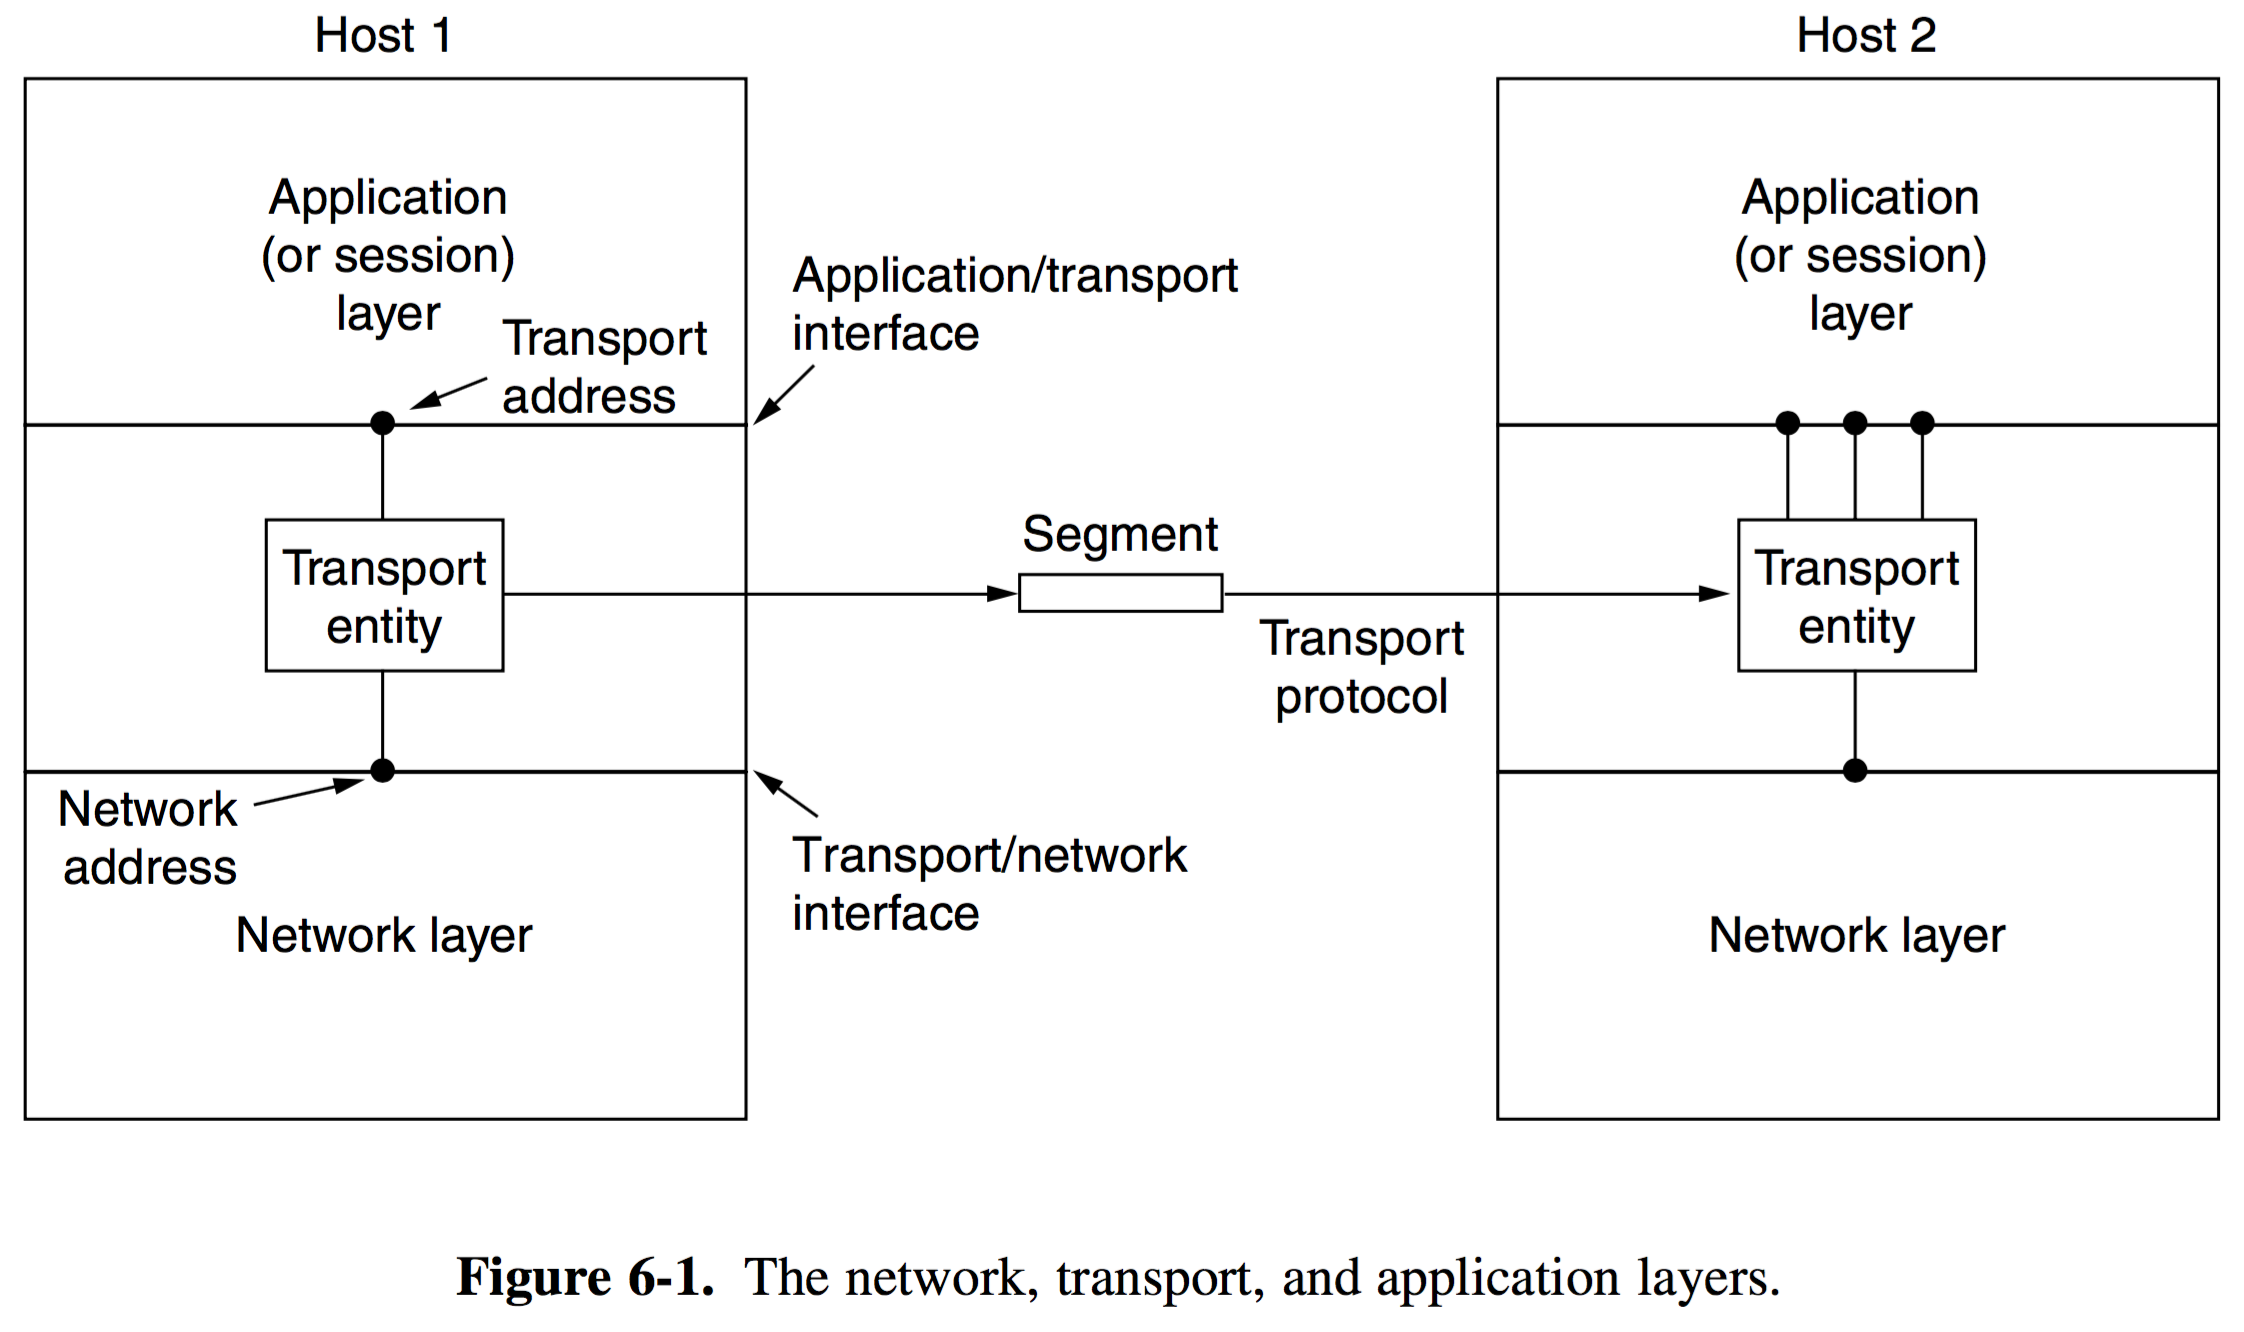
\includegraphics[width=8cm, height=5cm]{./imagenes/transporte.png} 
	\end{center}

\subsection{Primitivas del servicio de transporte}
\par Para permitir que los usuarios accedan al servicio de transporte, la capa de 
transporte debe proporcionar algunas operaciones a los programas de aplicación; es 
decir, una interfaz del servicio de transporte.

\begin{center}
	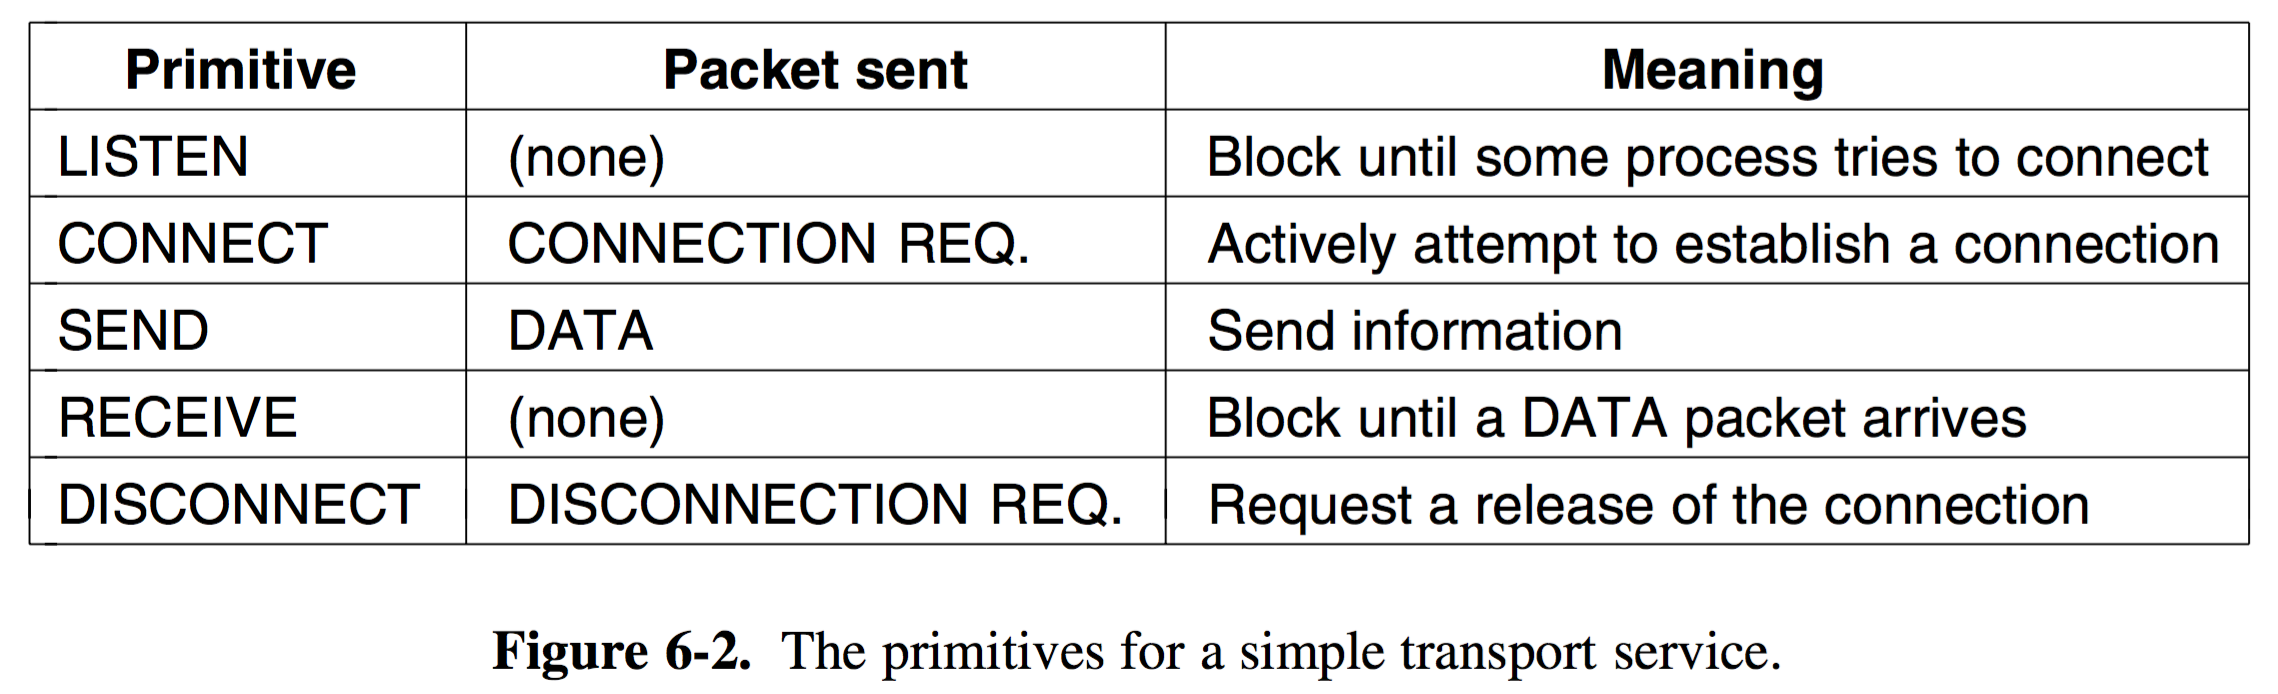
\includegraphics[width=11cm, height=5cm]{./imagenes/primitivas.png} 
\end{center}

\par Usaremos el término \textbf{segmento} para indicar los mensajes que se envían 
de una entidad de transporte a otra. Así, los segmentos (intercambiados por la capa 
de transporte) están contenidos en paquetes (intercambiados por la capa de red), y a 
su vez estos paquetes están contenidos en \textbf{tramas} (intercambiadas por la 
capa de enlace de datos).
\par Cuando llega una trama, la capa de enlace de datos procesa el encabezado de la 
trama y, si la dirección de destino coincide para la entrega local, pasa el contenido del 
campo de carga útil de la trama a la entidad de red. Esta úlltima procesa de manera 
similar el encabezado del paquete y después pasa el contenido de la carga útil del 
paquete a la entidad de transporte. 

\begin{center}
	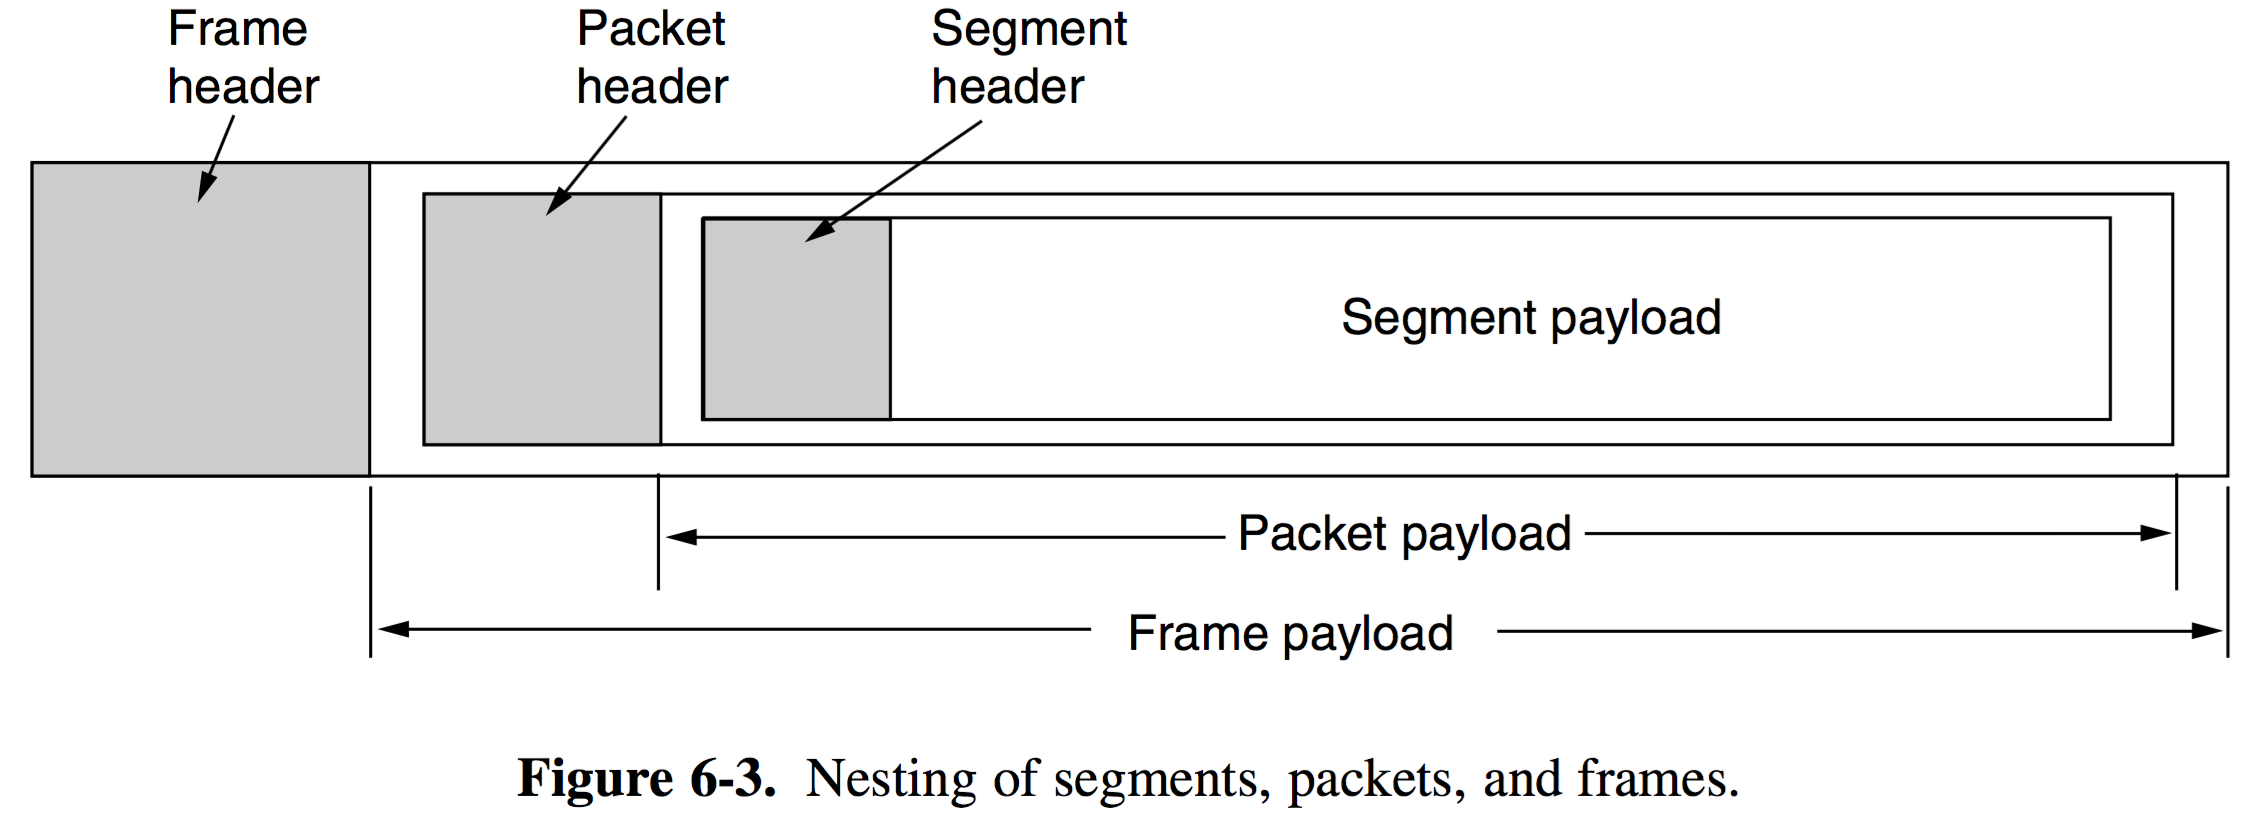
\includegraphics[width=8cm, height=4cm]{./imagenes/segmentos.png} 
\end{center}

\par Durante una conexión entre dos host se confirmará la recepción de cada 
paquete de datos enviado mediante las entidades de transporte, de manera 
transparente para los usuarios de transporte. De la misma forma, las entidades de 
transporte tienen que preocuparse por los temporizadores y las retransmisiones. Los 
usuarios de transporte no se enteran de ningún aspecto de esta mecánica. Para ellos 
una conexión es un conducto de bits confiable: un usuario mete bits en él y por arte 
de magia aparecen en el otro lado, con el mismo orden.

\par Veamos ahora un diagrama de estado para un esquema simple de manejo de 
conexiónes:

\begin{center}
	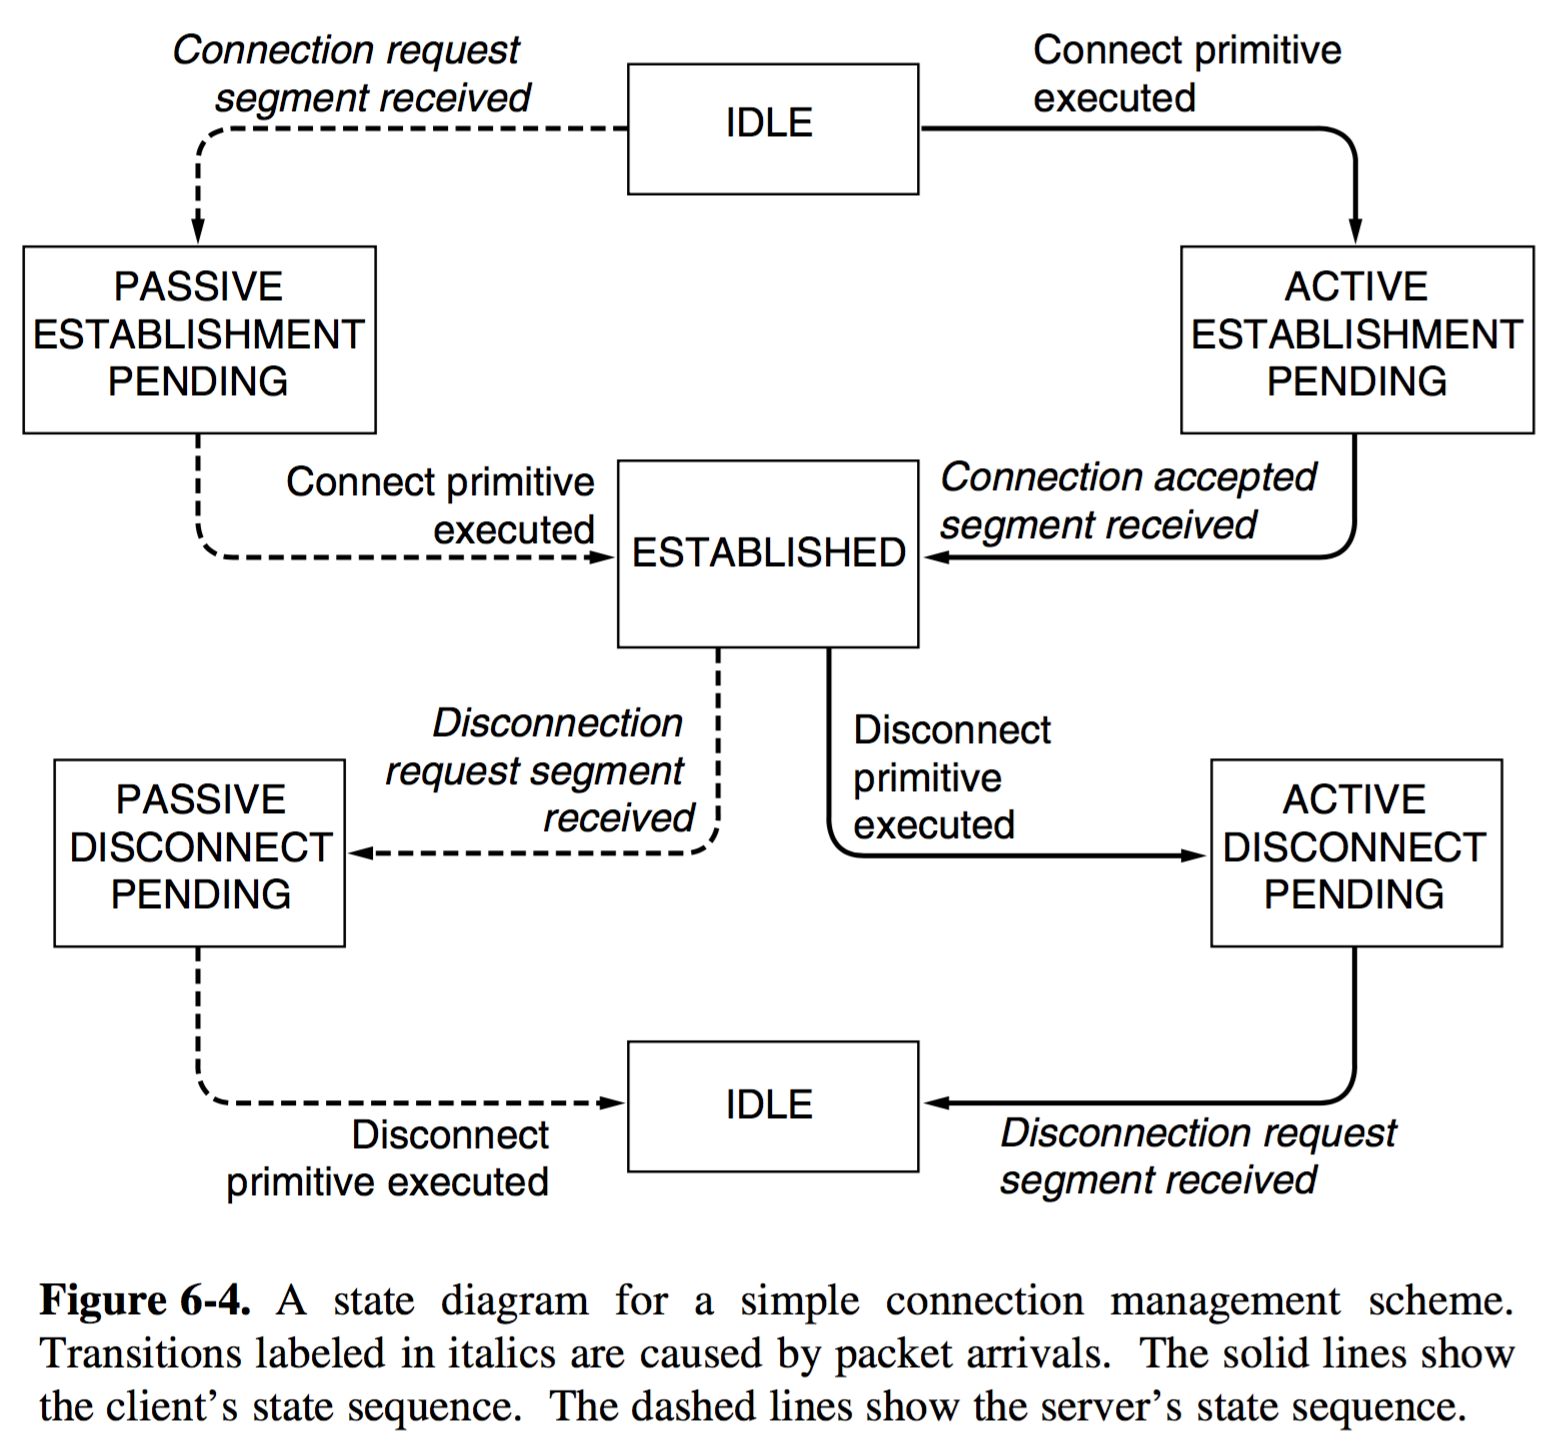
\includegraphics[width=11cm, height=7cm]{./imagenes/diagrama.png} 
\end{center}

\subsection{Sockets de Berkeley}


\section{Elementos de los protocolos de transporte}
\par El servicio de transporte se implementa mediante un \textbf{protocolo de 
transporte} entre las dos entidades de transporte. En la capa de transporte se requiere 
el direccionamiento explícito de los destinos, se requieren búferes y control de flujo.

\subsection{Direccionamiento}
\par Cuando un proceso de aplicación desea establecer una conexión con un proceso 
de aplicación remoto, debe especificar a cuáll se conectará. El método que se emplea 
por lo general es definir direcciones de transporte en las que los procesos puedan 
escuchar las solicitudes de conexión. En Internet, estos puntos terminales se 
denominan \textbf{puertos}. Usaremos el término genérico TSAP (Transport Service 
Access Point) para indicar un punto terminal específico en la capa de transporte. Los 
puntos terminales análogos en la capa de red (es decir, direcciones de capa de red) se 
llamen NSAP (Network Service Access Points). Las direcciones IP son ejemplos de 
NSAP.
\par Los procesos de aplicación,tanto clientes como servidores, se pueden enlazar por 
si mismos a un TSAP para establecer una conexión a un TSAP remoto. Estas 
conexiónes se realizan a través de NSAPs en cada host. Los TSAPs sirven para 
distinguir los múltiples puntos terminales de transporte que comparten un NSAP.

\begin{center}
	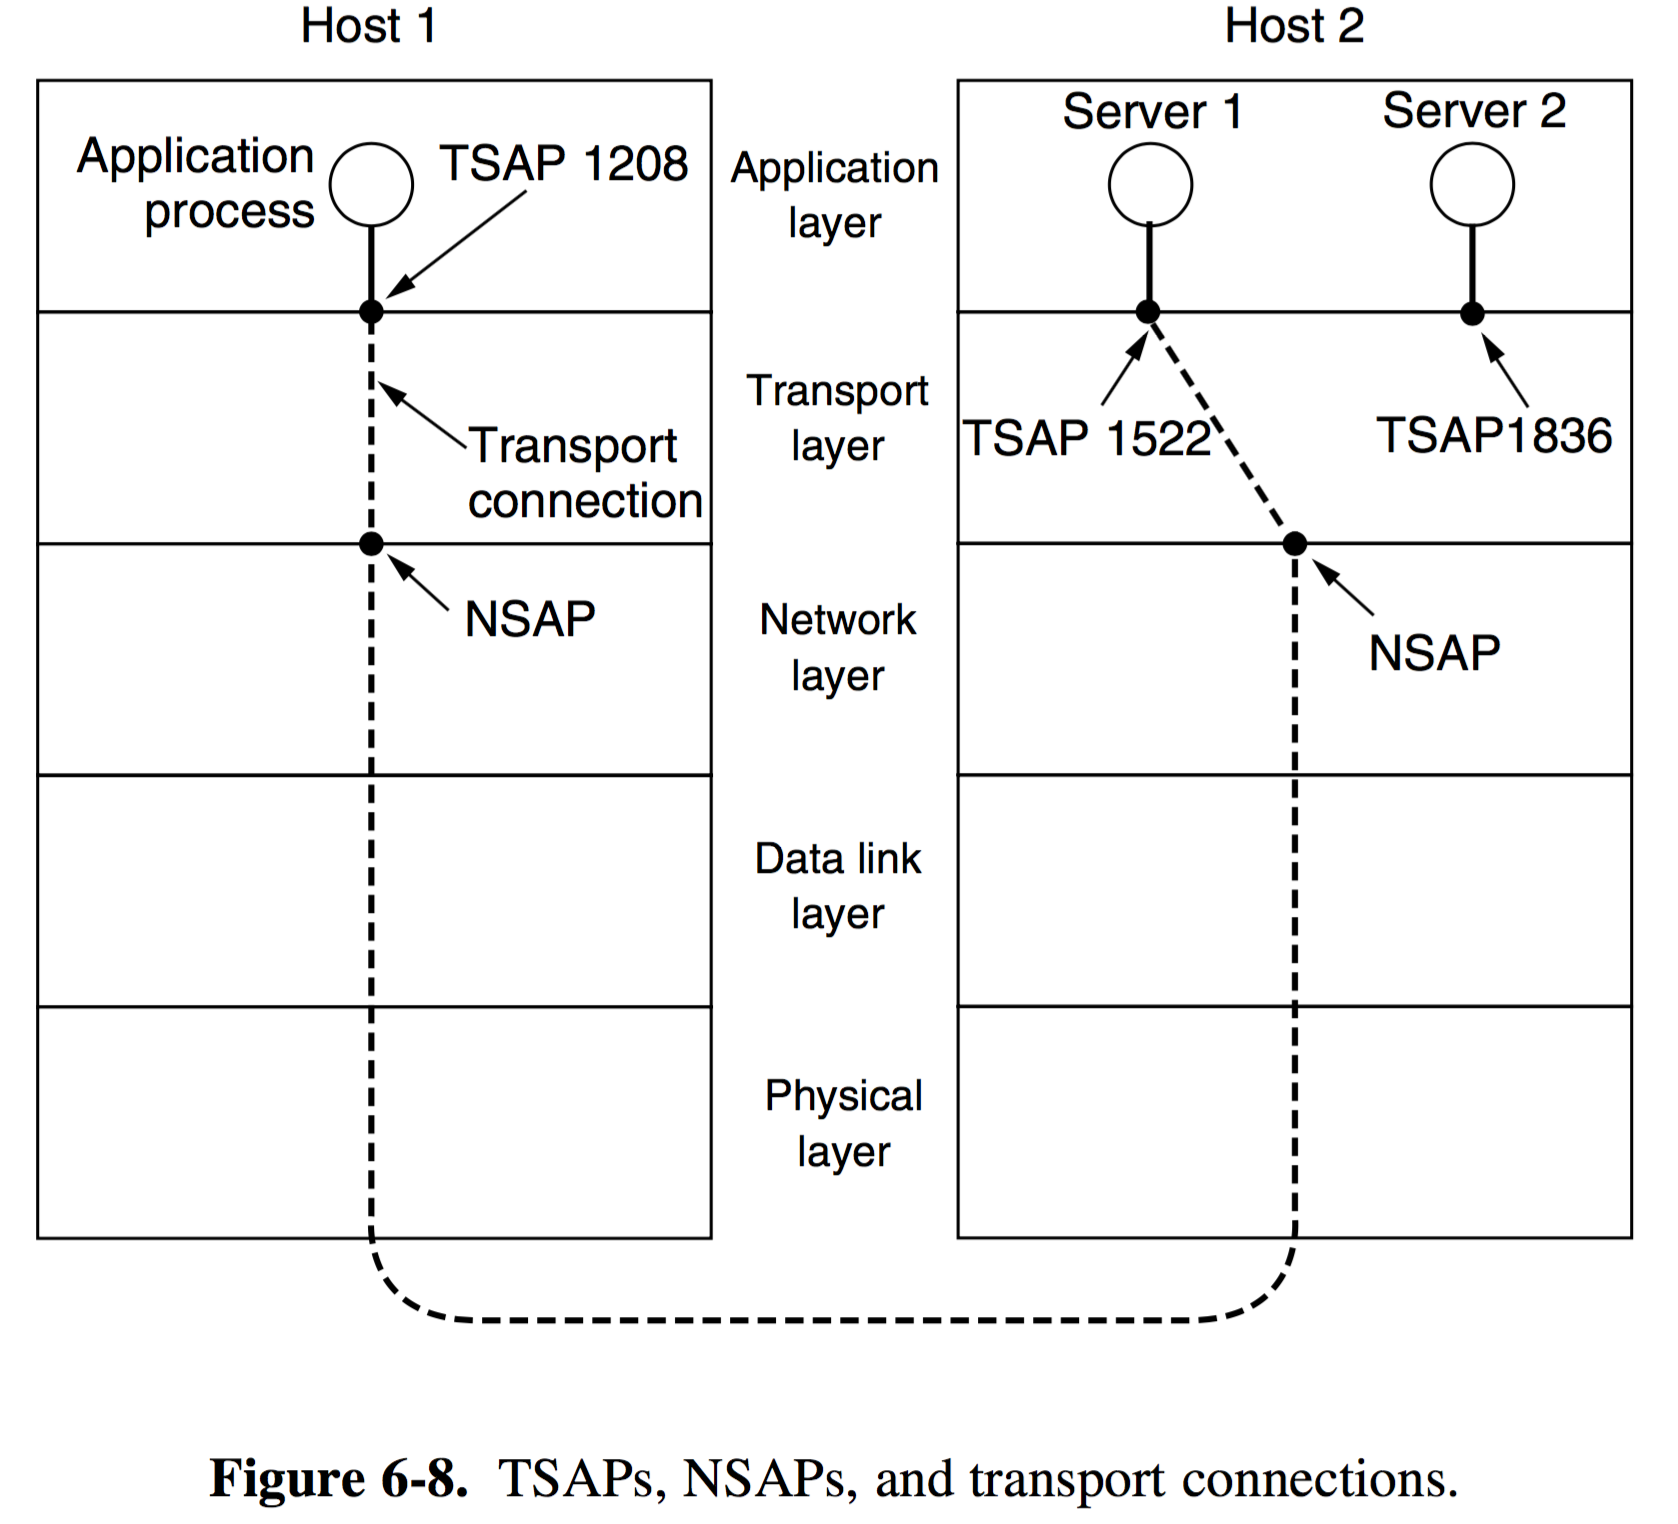
\includegraphics[width=6cm, height=5cm]{./imagenes/tsap.png} 
\end{center}

\par ¿Cómo sabe un proceso de usuario que un servidor \textbf{\textit{S}} está 
conectado a un determinado TSAP?

\begin{itemize}
	\item \underline{Solución 1:} una posibilidad es que S se ha estado conectando al 
	mismo TSAP durante años y gradualmente todos los usuarios de la red han 
	aprendido esto. En este modelo los servicios tienen direcciones TSAP estables que 
	se listan en archivos en lugares bien conocidos.
	\par Los procesos de usuario frecuentemente desean comunicarse con otros 
	procesos de usuario que solo existen durante un tiempo corto y no tienen una 
	dirección TSAP conocida por adelantado. En el caso de que hubiese muchos 
	procesos de servidor, la mayoría de los cuales se usaran pocas veces sería un 
	desperdicio tenerlos activados a todos escuchando en una dirección TSAP estable 
	todo el día.
	\item \underline{Solución 2:} un esquema alternativo en forma simplificada, es el 
	conocido como \textbf{protocolo inicial de conexión}. Cada máquina que desea 
	ofrecer servicios a usuarios remotos tiene un servidor de procesos especial que 
	actúa como 	proxy de los servidores de menor uso. Este servidor es llamado 
	\textit{inetd} en sistemas UNIX; el mismo escucha en un grupo de puertos al mismo 
	tiempo esperando una solicitud de conexión. Los usuarios potenciales de un 
	servicio comienzan por emitir una solicitud 	\textbf{CONNECT}, especificando la 
	dirección	TSAP del servicio que desean, si no hay ningún servidor esperándolos, 
	consiguen una conexión al servidor de procesos.
	 \par Tras obtener la solicitud entrante el servidor de procesos genera el servidor 
	 solicitado, permitiéndole heredar la conexión con el usuario existente. El nuevo 
	 servidor entonces hace el trabajo requerido, mientras que el servidor de procesos 
	 retorna a escuchar solicitudes nuevas.
	\par Hay muchas situaciones en las que los servicios existen independientemente 
	del servidor de procesos. Por ejemplo, un servidor de archivos necesita operar en un 
	hardware especial (una máquina con un disco) y no puede crearse simplemente 
	sobre la marcha cuando alguien quiere comunicarse con él.
	
	\begin{center}
	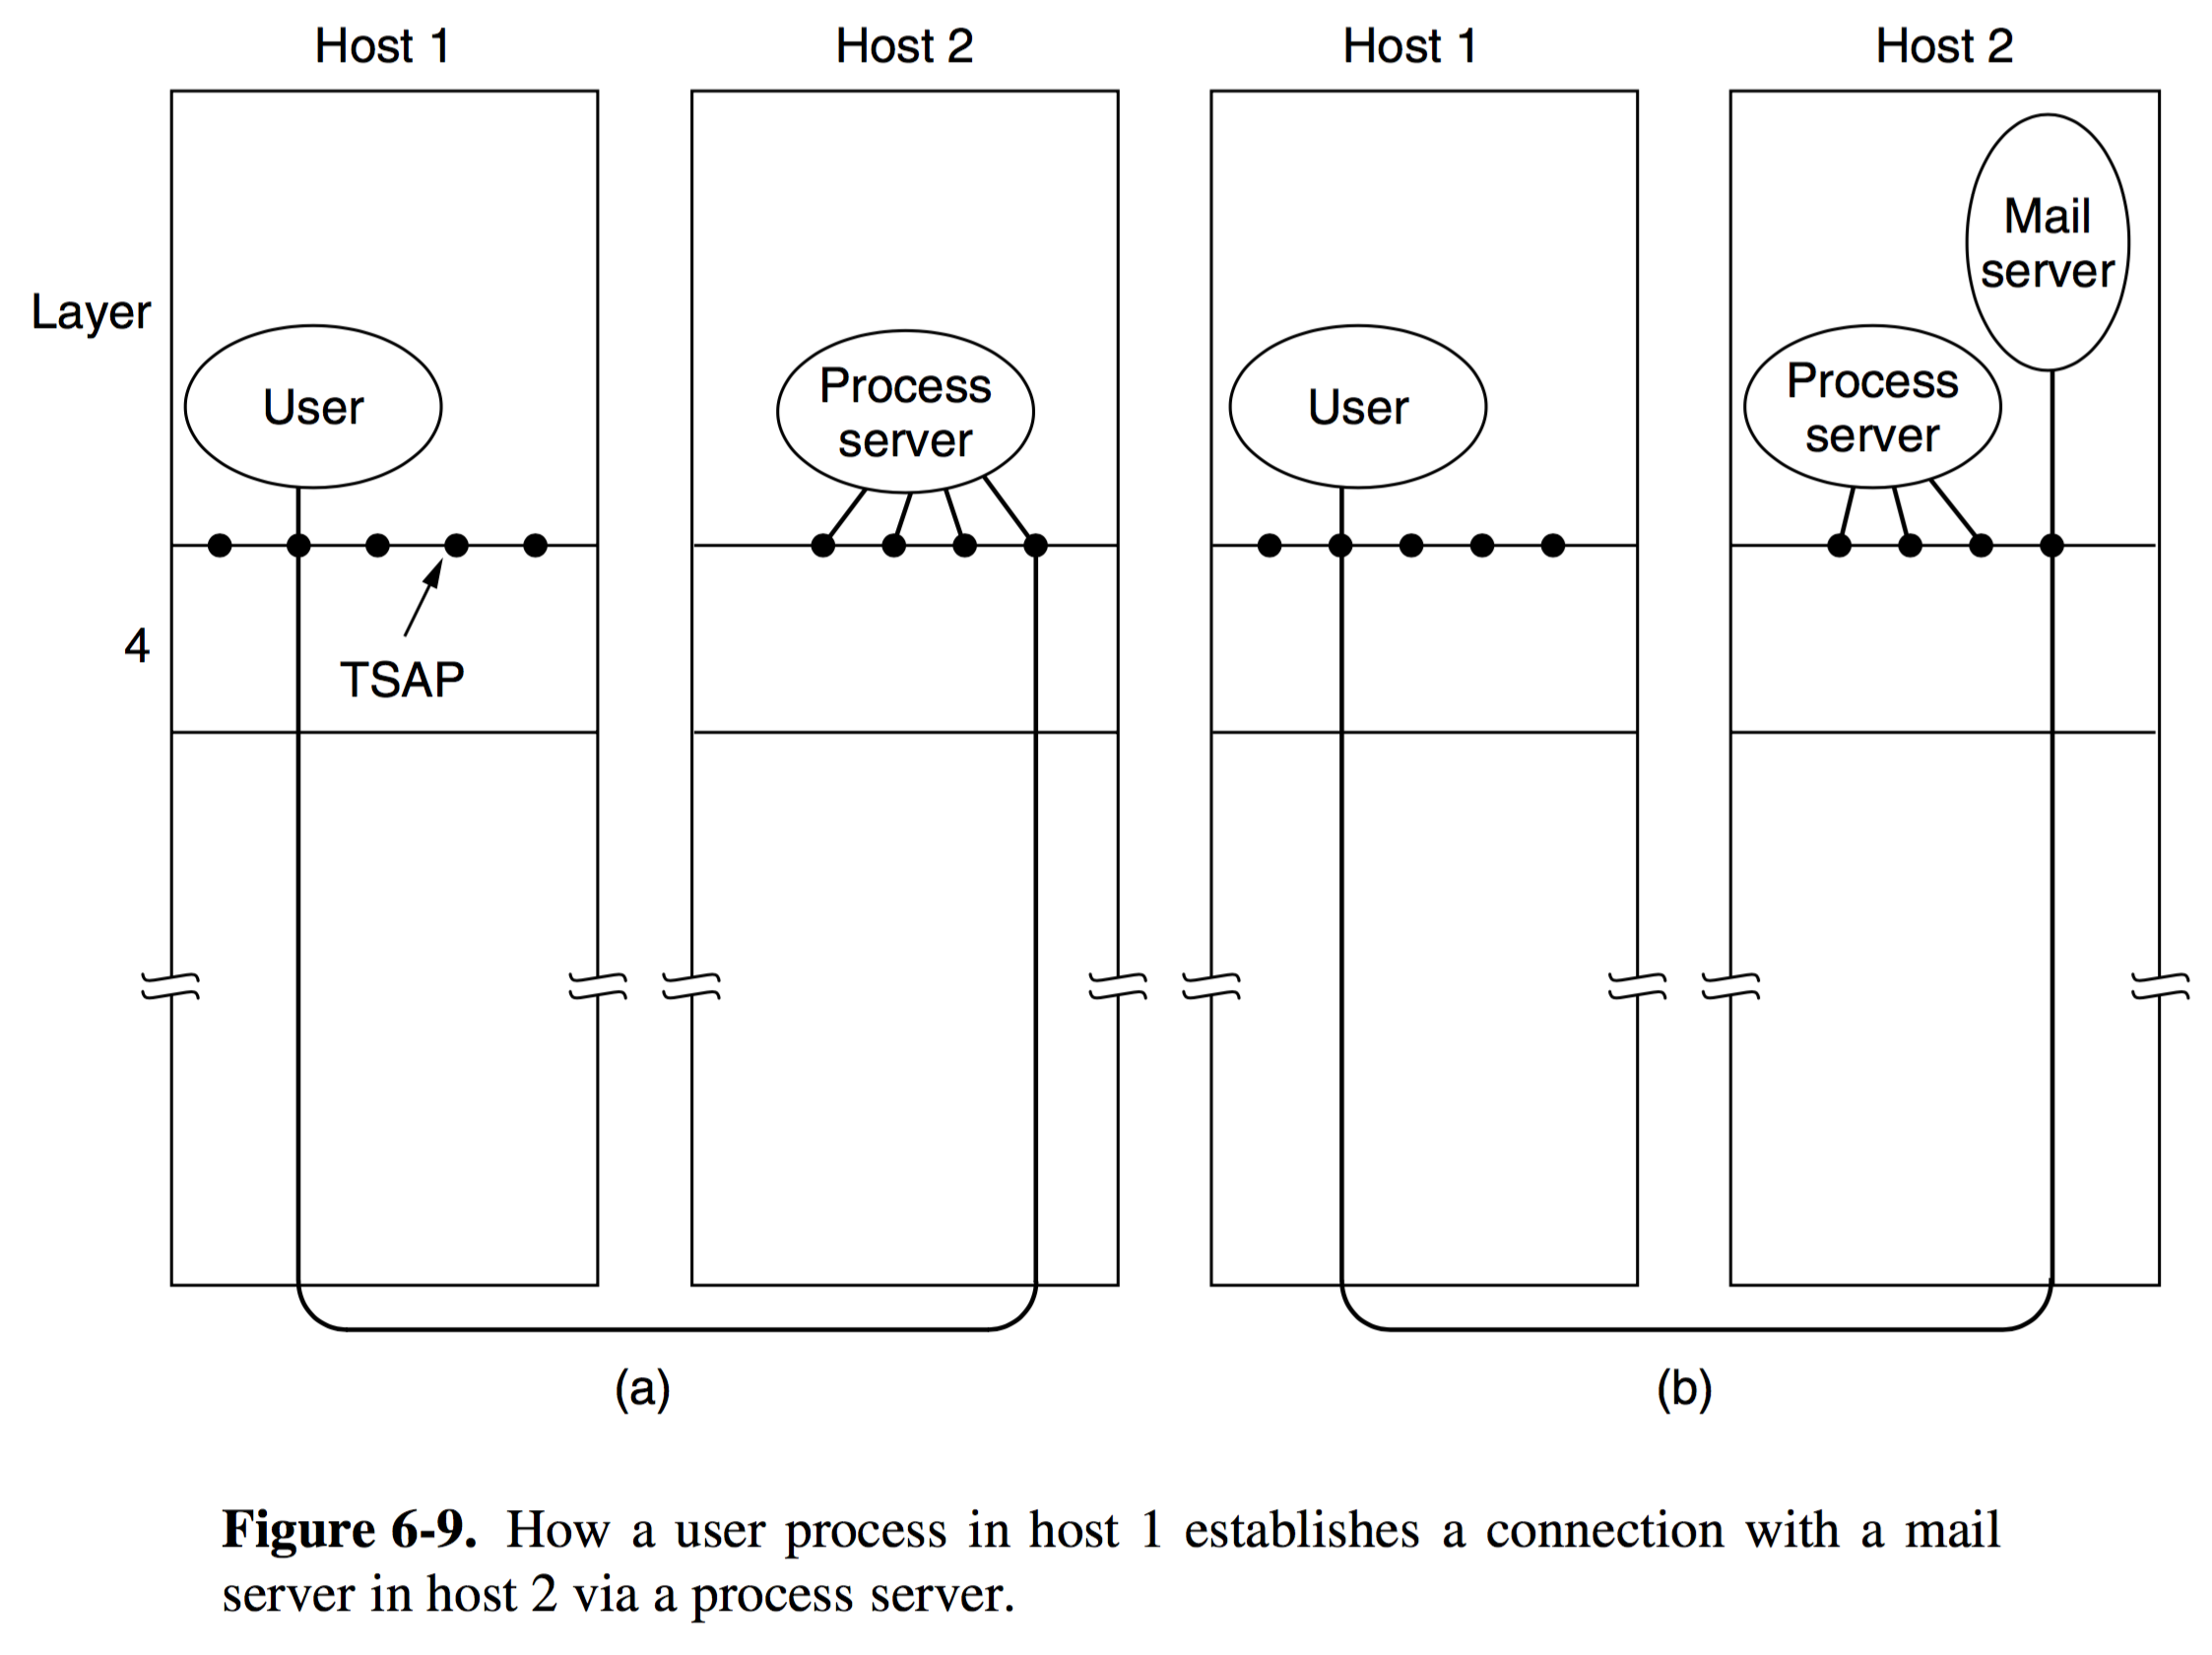
\includegraphics[width=9cm, height=6cm]{./imagenes/conexioninicial.png} 
	\end{center}

	\item  \underline{Solución 3:} Existe un proceso especial llamado \textbf{servidor 
	de nombres} (también llamado servidor de directorio); para encontrar la dirección 
	TSAP correspondiente a un nombre de servicio dado, el usuario establece una 
	conexión con el servidor de nombres (que escucha en un TSAP bien conocido). 
	Entonces el 	usuario envía un mensaje especificando el nombre del servicio y el 
	servidor de nombres le devuelve la dirección TSAP, luego el usuario libera la 
	conexión con el servidor de nombres y establece una nueva con el servicio deseado. 
	Al crearse un servicio nuevo debe registrarse en el servidor de nombres, dando su 
	nombre de servicio como la dirección de su TSAP. El servidor de nombres registra 
	esta 	información en su base de datos.
\end{itemize} 

\subsection{Establecimiento de una conexión}

\subsection{Liberación de una conexión}

\subsection{Control de errores y almacenamiento en búfer}
\subsection{Multiplexión}
\subsection{Recuperación de fallas}
\section{Control de congestión}
\subsection{Asignación de ancho de banda deseable }
\subsection{Regulación de la tasa de envío}
\subsection{Cuestiones inalámbricas}
\section{Los protocolos de transporte de internet: UDP}
\subsection{Introducción a UDP}
\subsection{Llamada a procedimiento remoto}
\subsection{Protocolos de transporte en tiempo real}


\section{Los protocolos de transporte de internet: TCP}

\subsection{Introducción a TCP}
\par La mayoría de las aplicaciones en internet necesitan una entrega en secuencia 
confiable, para ellos se diseñó \textbf{TCP (Transmission Control Protocol)} que sirve 
para proporcionar un flujo de bytes confiable de extremo a extremo a través de una 
interred no confiable. TCP tiene un diseño que se adapta de manera dinámica a las 
propiedades de la interred y que se sobrepone a muchos tipos de fallas.
\par Cada máquina que soporta TCP tiene una entidad de transporte TCP (ETCP), ya 
sea un procedimiento de biblioteca, un proceso de usuario, o parte del kernel. En todos 
los casos maneja flujos TCP e interactúa con la capa IP. Una ETCP acepta flujos de 
datos de usuario de procesos locales, los divide en fragmentos que no excedan los 64 
KB, y envía cada fragmento como un datagrama IP independiente. Cuando los 
datagramas que contienen datos TCP llegan a una máquina, se pasan a la ETCP, la cual 
reconstruye los flujos de bytes originales. Usaremos la palabra TCP para referirnos: a 
veces a la ETCP y a veces al protocolo TCP.
\par La capa IP no proporciona ninguna garantía de que los datagramas se entregarán 
de manera apropiada, por lo que corresponde a TCP terminar los temporizadores y 
retransmitir los datagramas conforme sea necesario.
\par Los datagramas que llegan podrán hacerlo en el orden incorrecto, esto sucede 
cuando se trabaja con redes de datagramas. Corresponde a TCP reensamblarlos en 
mensajes en la secuencia apropiada ya que usualmente la capa de aplicación del 
receptor necesita procesar los mensajes en el orden en que fueron enviados.

\subsection{El modelo del servicio TCP}
\par El servicio TCP se obtiene al hacer que tanto el servidor como el cliente creen 
puntos terminales llamados \textbf{\textit{sockets}}. Cada socket tiene una dirección 
que consiste en la dirección IP del host, y un número de 16 bits llamado \textbf{puerto}, el cual es local a ese host. Un puerto es el nombre TCP para un TSAP.
\par Para obtener el servicio TCP se debe establecer de manera explícita una conexión entre el socket en la máquina emisora y uno en la máquina receptora. Un socket puede usarse para múltiples conexiones al mismo tiempo, dos o más conexiones pueden terminar en el mismo socket. Las conexiones se identifican mediante los identificadores de sockets de los dos extremos, es decir (socket1, socket2).
\par Todas las conexiones TCP son de dúplex total y de punto a punto.
	\begin{itemize}
		\item Dúplex total: el tráfico puede ir en ambas direcciones al mismo tiempo.
		\item Punto a punto: cada conexión tiene exactamente dos puntos finales.
		\item  TCP no soporta la multidifusión ni la difusión.
	\end{itemize}
\par Una conexión TCP es un flujo de bytes, no un flujo de mensajes. Los límites de los 
mensajes no se preservan de extremo a extremo.

\textbf{Ejemplo:} el proceso emisor realiza 4 escrituras de 512 B en el flujo TCP, tal 
vez estos datos se entreguen al proceso receptor como 4 fragmentos de 512 B, o dos 
fragmentos de 1024 B, o uno de 2048 B o de alguna otra forma.

	\begin{center}
	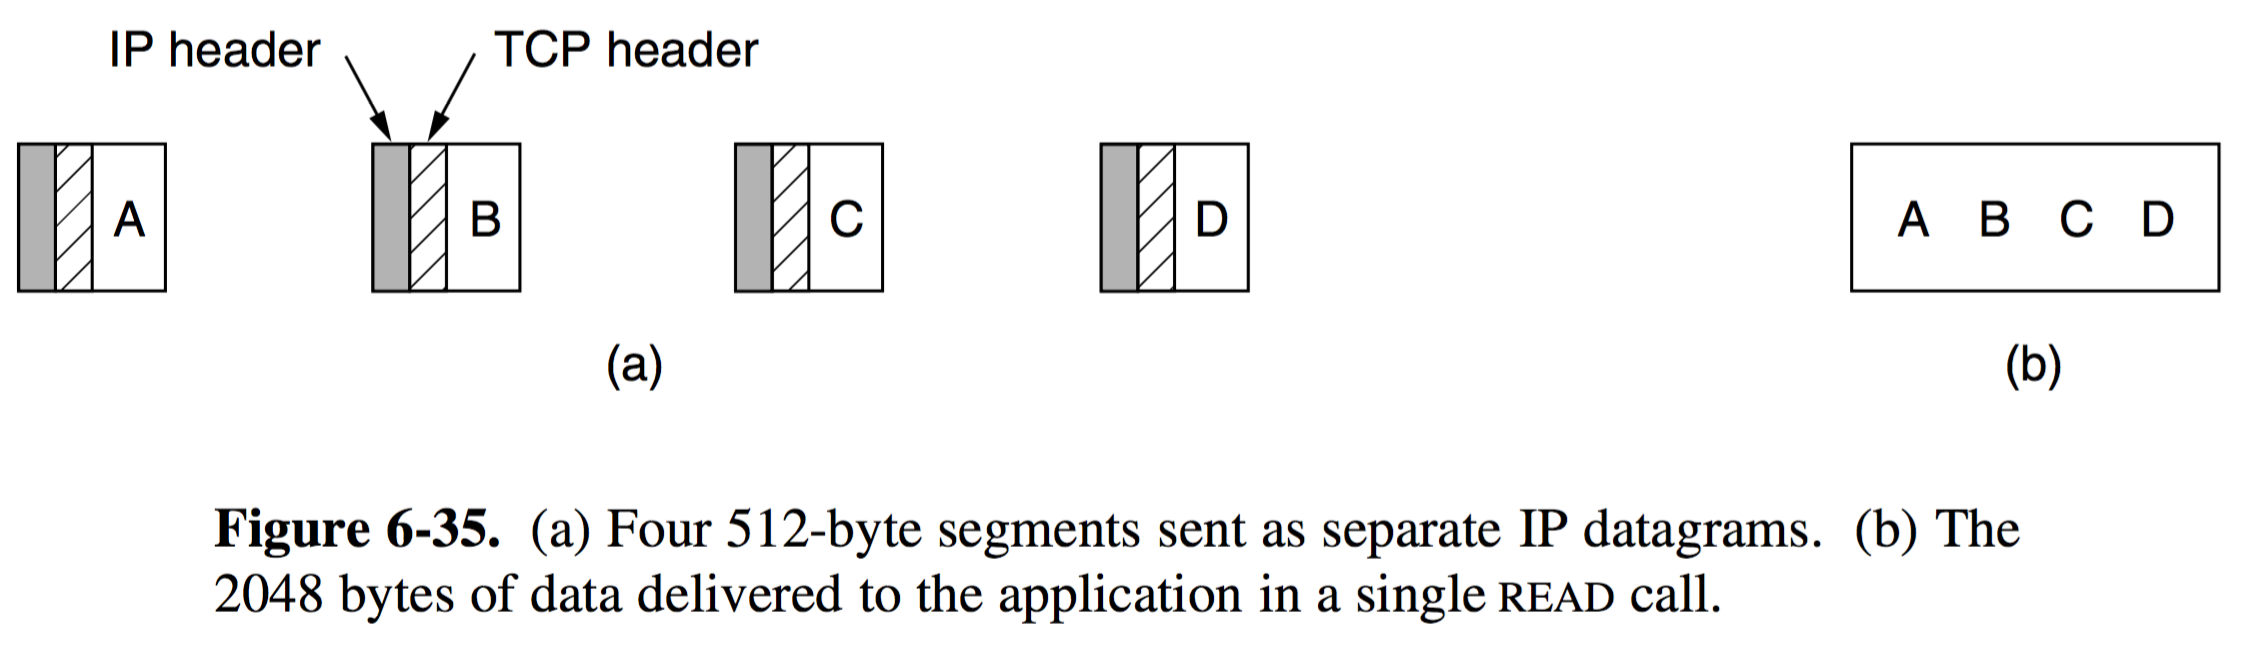
\includegraphics[width=14cm, height=4cm]{./imagenes/tcp.png} 
	\end{center}

\par No hay manera que el receptor detecte las unidades en las que se escribieron los 
datos. El software TCP no tiene idea de lo que significan los bytes y no le interesa 
averiguarlo.

\par Cuando una aplicación pasa datos a TCP, este decide si los envía inmediatamente 
o si los almacena en el búfer a fin de recolectar una gran cantidad y luego enviarlos al 
mismo tiempo. Sin embargo la aplicación algunas veces necesita que los datos se 
envíen de inmediato.

\textbf{Ejemplo:} si un usuario inicia una sesión con una máquina remota. Una vez que 
se termina una línea de comandos y se introduce un retorno de carro es esencial que la 
línea se envíe a la máquina remota inmediatamente y que no se almacene en el búfer 
hasta que llegue la siguiente línea. Para obtener los datos, las aplicaciones pueden 
utilizar el indicador \textbf{PUSH} que es una señal para TCP de que no debe retrasar 
la transmisión, si llegan indicadores PUSH antes de que el primero se haya transmitido 
(por ejemplo, debido a que la línea de salida está ocupada), TCP es libre de recolectar 
todos los datos con indicadores PUSH en un solo datagrama IP, sin ninguna separación 
entre las diversas piezas.

Cuando un usuario interactivo oprime las teclas \emph{Ctrl+C} o \textit{Supr} para 
interrumpir una operación remota que ha iniciado, la aplicación emisora coloca 
información de control en el flujo de datos y se la da a TCP junto con el indicador 
\textbf{URGENT}. Este evento ocasiona que TCP interrumpa el encolamiento de datos 
y transmita inmediatamente todo lo que tenga para esa conexión. Cuando el destino 
recibe los datos urgentes, se interrumpe la aplicación receptora, a fin de que pueda 
detener lo que está haciendo y que lea el flujo de datos para leer los datos urgentes.
El final de los datos urgentes se marca para que la aplicación sepa dónde terminan.
El inicio de estos no se marca; la aplicación tiene que averiguarlo.

\subsection{Direccionamiento en TCP}
\par Los numeros de puerto menores que 1024 están reservados para los servicios 
estándar que, por lo general, sólo los usuarios privilegiados pueden iniciar. Éstos se 
llaman \textbf{puertos bien conocidos}.

	\begin{center}
	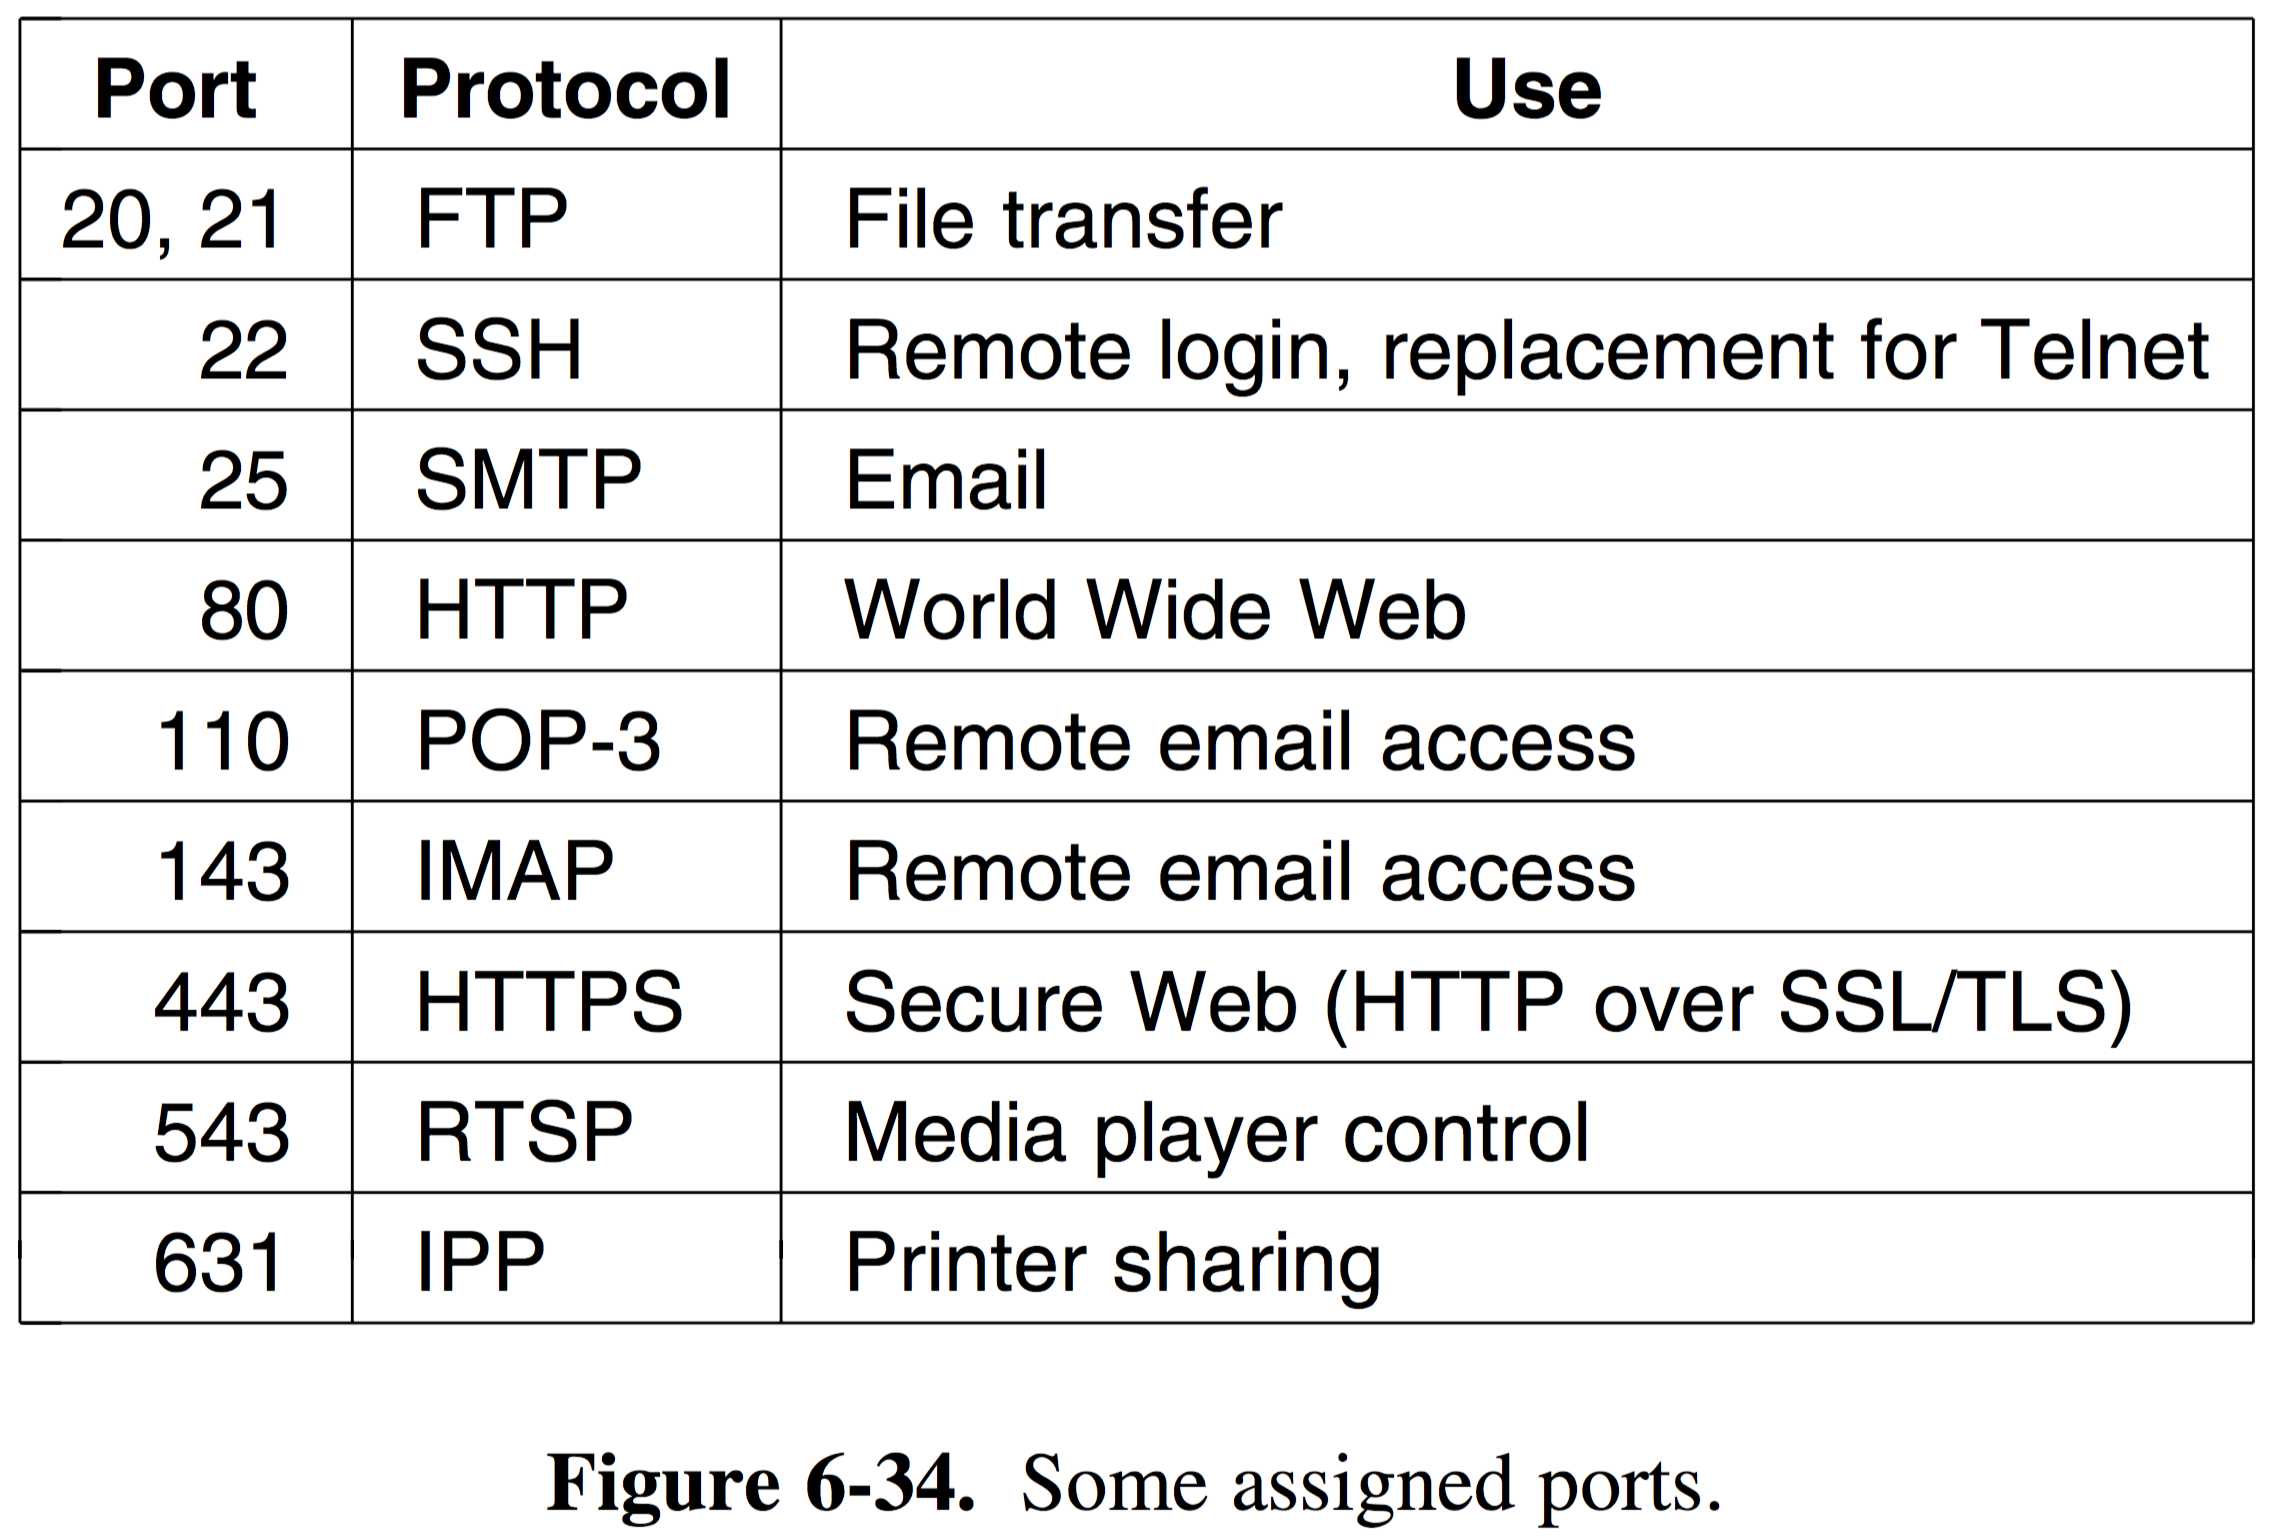
\includegraphics[width=9cm, height=6cm]{./imagenes/protocolo.png} 
	\end{center}

\par Podría ser posible que el demonio FTP se conecte por sí solo al puerto 21 en 
tiempo de arranque, que el demonio SSH se conecte por sí solo al puerto 22 en tiempo 
de arranque, y así en lo sucesivo. Sin embargo, hacer lo anterior podría llenar la 
memoria con demonios que están inactivos la mayor parte del tiempo. En su lugar, lo 
que se hace por lo general es que un solo demonio, llamado \emph{demonio de 
Internet (inetd)}, se conecte por sí solo a múltiples puertos y espere la primera 
conexión entrante. Cuando eso ocurre, \emph{inetd} bifurca un nuevo proceso y 
ejecuta el demonio apropiado en él, para dejar que ese demonio maneje la solicitud. De 
esta forma, los demonios distintos a \textit{inetd} sólo están activos cuando hay 
trabajo para ellos. \emph{Inetd} consulta un \textbf{archivo de configuración} para 
saber cuál puerto utilizar. El administrador del sistema puede 
configurar el sistema para tener demonios permanentes en los puertos más ocupados 
e \emph{inetd} en los demás.

\subsection{El protocolo TCP}
\par Cada byte de una conexión TCP tiene su propio número de secuencia de 32 bits. 
Los múmeros de secuencia separados de 32 bits se usan para confirmaciones de 
recepción y para el mecanismo de ventana. La entidad TCP emisora y la receptora 
intercambian datos en forma de segmentos. Un segmento consiste en un encabezado 
TCP fijo de 20 bytes (más una parte opcional) seguido de 0 o más bytes de datos. El 
software de TCP decide el tamaño de los segmentos; puede acumular datos de varias 
escrituras para formar un segmento, o dividir los datos de una escritura en varios 
segmentos.
\par Hay dos límites que restringen el tamaño de segmento:
	\begin{itemize}
		\item Cada segmento incluido el encabezado TCP, debe caber en la carga útil de 
		65.515 bytes del IP.
		\item Cada red tiene una unidad máxima de transferencia (MTU) y cada segmento 
		debe caber en la MTU.
		\item En la práctica la MTU es generalmente de 1500 bytes (el tamaño de la 
		carga útil de Ethernet).
	\end{itemize}	 
\par Cuando un transmisor envía un segmento, también inicia un temporizador. Cuando 
llega el segmento a destino, la ETCP receptora devuelve un segmento (con datos si 
existen, de otro modo sin ellos) que contiene un número de confirmación de recepción 
igual al siguiente número de secuencia que espera recibir. Si el temporizador del emisor 
expira antes de la recepción de la confirmación, el emisor envía de nuevo el segmento.

\subsubsection{Problemas a manejar/resolver por TCP eficientemente:}
\begin{itemize}
	\item Pueden llegar segmentos fuera de orden, por lo que los bytes 3072-4095 
	podrían llegar pero no enviarse confirmación de recepción, porque los bytes 
	2048-3071 no han aparecido aún.
	\item También pueden retardarse segmentos en tránsito durante tanto tiempo que 
	el temporizador del emisor expira y los segmentos se retransmiten.
	\item Las retransmisiones podrían incluir rangos de bytes diferentes a los de la 
	transmisión original, lo cual requiere una administración cuidadosa para llevar el 
	control de los bytes que se han recibido correctamente en un momento 
	determinado. Esto es factible ya que cada byte del flujo tiene su propio
	desplazamiento único.
\end{itemize}

\subsection{El encabezado del segmento TCP}
\par En la figura 6-36 se muestra la distribución de un segmento TCP. Cada segmento 
comienza con un encabezado de formato fijo de 20 bytes. El encabezado fijo puede ir 
seguido de encabezado de opciones. Después de las opciones, si las hay, pueden 
continuar hasta 65535$-$20$-$20$=$65495 bytes de datos, donde los primeros 20 se 
refieren al encabezado IP y los segundos al encabezado TCP. Los segmentos sin datos 
son legales y se usan por lo común para confirmaciones de recepción y mensajes de 
control.

	\begin{center}
	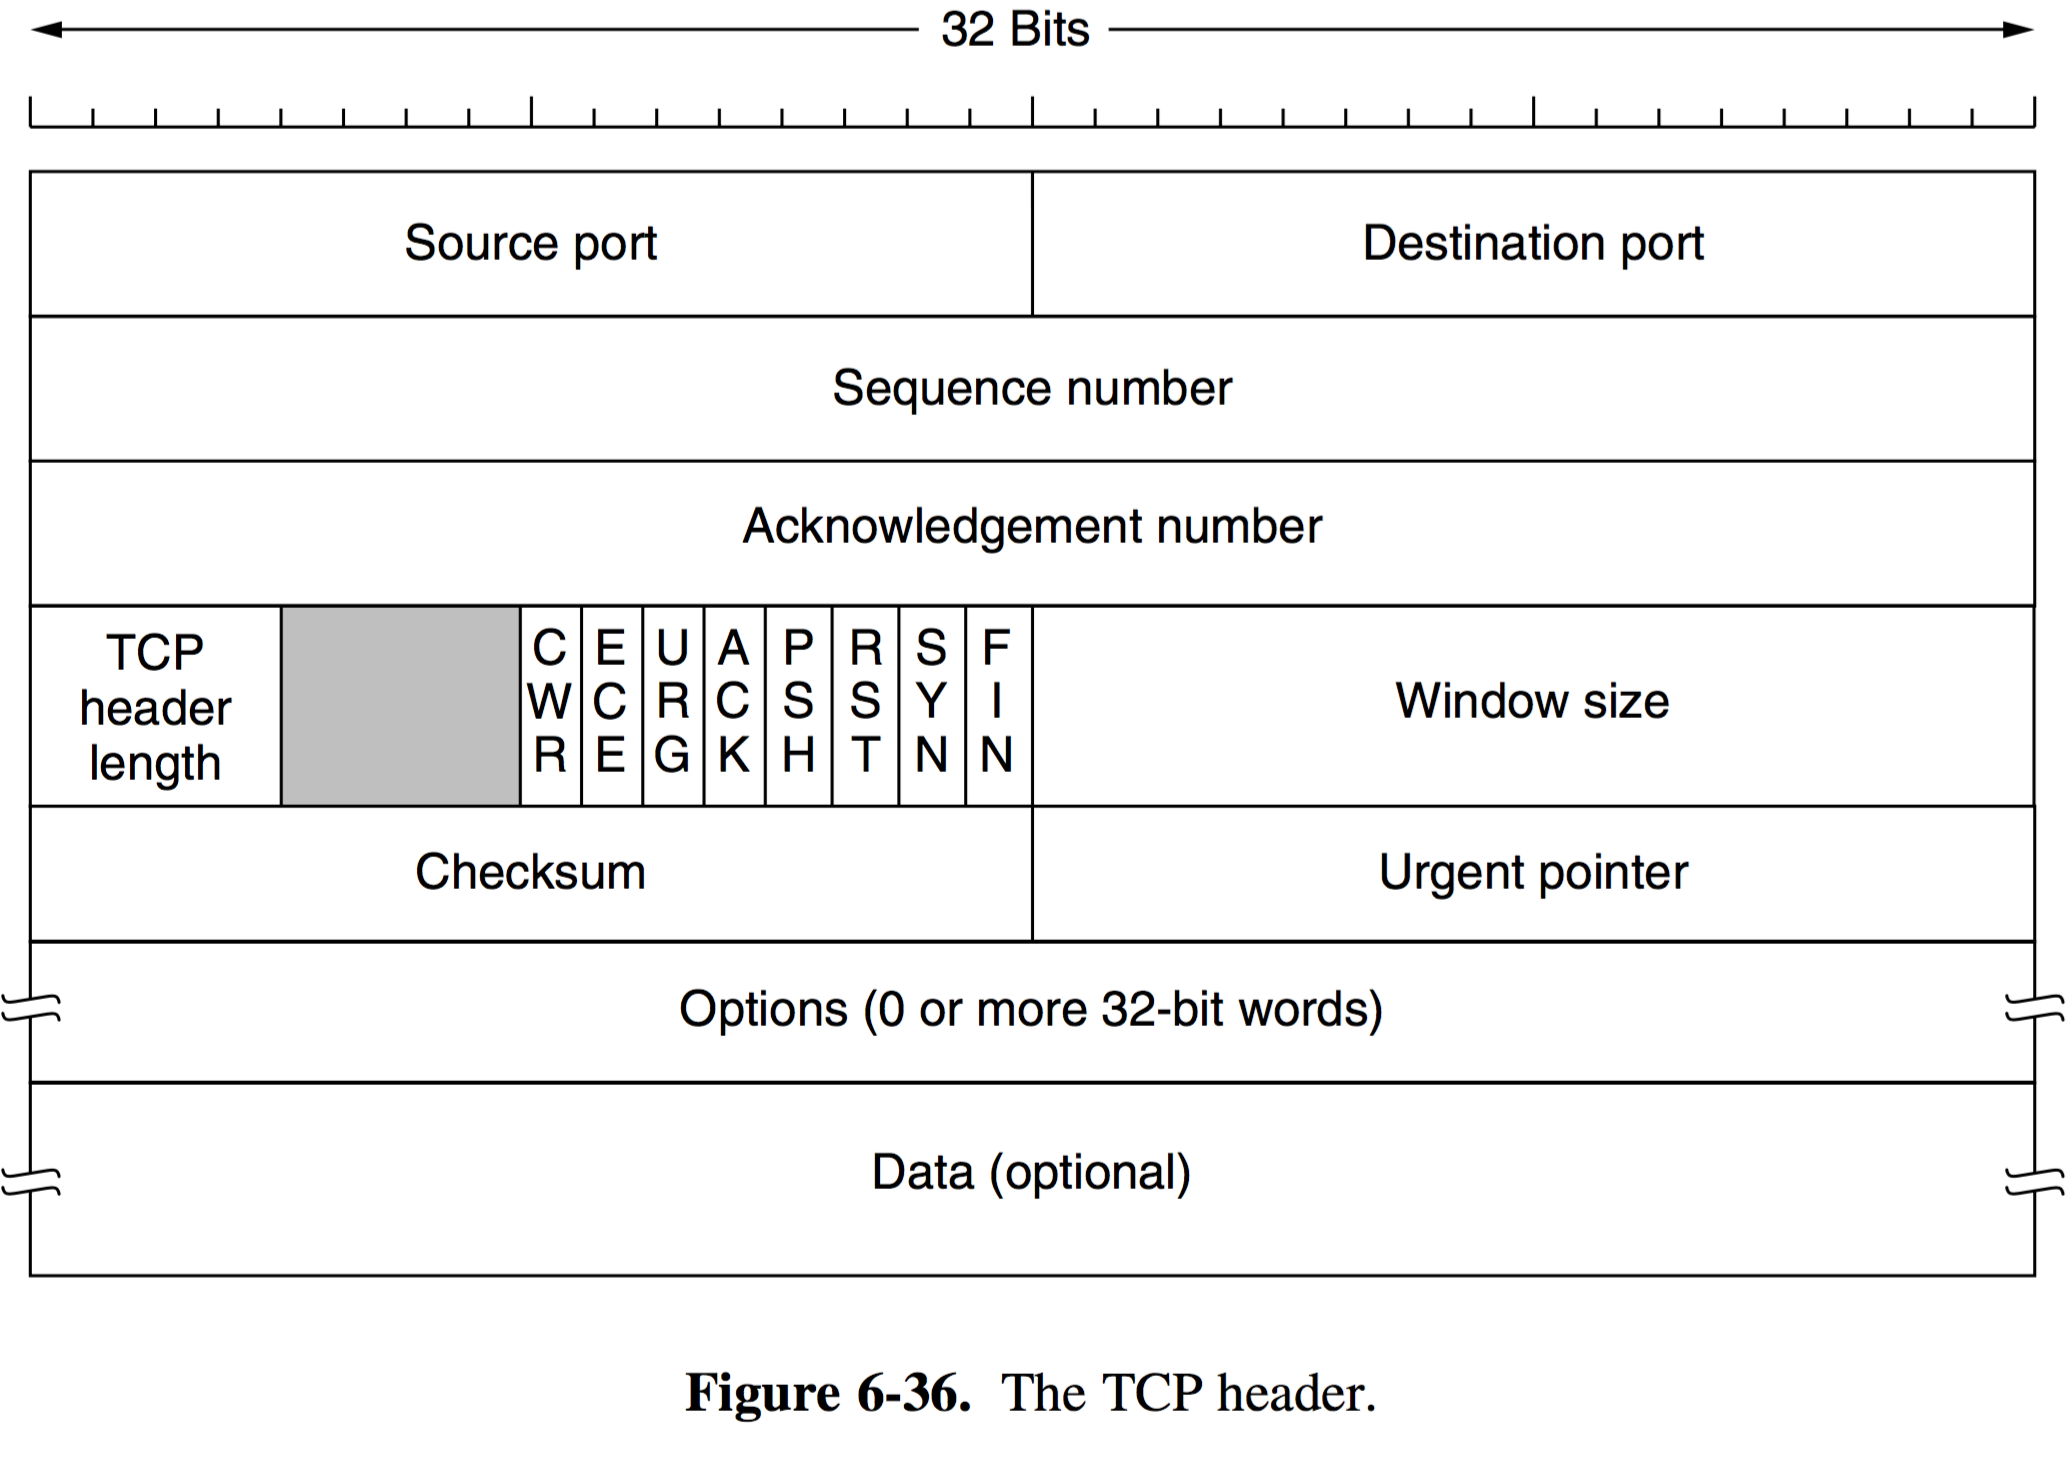
\includegraphics[width=9cm, height=6cm]{./imagenes/encabezado.png} 
	\end{center}

\par Los campos de \textit{puerto de origen} y \textit{puerto de destino} identifican 
los puntos terminales locales de la conexión. La dirección de un puerto más la dirección 
IP del host forman un punto terminal único de 48 bits. Los puntos terminales de origen 
y de destino en conjunto identifican la conexión.
\par Los campos \textit{número de secuencia} y \textit{número de confirmación de 
recepción} desempeñan sus funciones normales. El segundo indica el siguiente byte 
esperado, no el último byte correctamente recibido. Ambos tienen 32 bits de longitud porque cada byte de datos está numerado en el flujo TCP.
\par La \textit{longitud del encabezado TCP} indica la cantidad de palabras de 32 
bits contenidas en el encabezado TCP. Esta información es necesaria porque el campo 
\textit{Opciones} es de longitud variable, por lo que el encabezado también. Este 
campo indica el comienzo de los datos en el segmento, medido en palabras de 32 bits, 
pero ese número es simplemente la longitud del encabezado en palabras. A 
continuación viene un campo de 6 bits que no se usa.
\par Luego vienen 8 indicadores de 1 bit:
	\begin{itemize}
		\item \textbf{CWR} y \textit{ECE} se utilizan para indicar congestión cuando se 
		usa ECN (Notificación Explícita de Congestión). ECE se establece para indicar una 
		\textit{ECN-Echo} a un emisor TCP y decirle que reduzca su velocidad cuando el 
		receptor TCP recibe una indicación de congestión de la red. CWR se establece 
		para indicar una \textit{Ventana de congestión} reducida del emisor TCP al 
		receptor TCP, de modo que sepa que el emisor redujo su velocidad y puede dejar 
		de enviar la \textit{Repetición de ECN}.
		\item \textbf{URG} se establece en 1 si está en uso el \textit{Apuntador Urgente}, el cual 
		sirve para indicar un desplazamiento en bytes a partir del número actual de 
		secuencia en el que se encuentran datos urgentes, sustituye los mensajes de 
		interrupción y un mecanismo rudimentario para permitir que el emisor envíe una 
		señal al receptor sin implicar al TCP en la razón de la interrupción.
		\item \textbf{ACK} se establece en 1 para indicar que el \textit{Número de confirmación 
		de recepción} es válido. Si es 0, el segmento no contiene una confirmación de 
		recepción, por lo que se ignora el campo de número de confirmación de 
		recepción.
		\item \textbf{PSH} indica datos que se deben transmitir de inmediato. Por este medio se 
		solicita atentamente al receptor que entregue los datos a la aplicación a su 
		llegada y no los almacene en búfer hasta la recepción de un búfer completo.
		\item \textbf{RST} se usa para restablecer de manera repentina una conexión 
		que se ha confundido debido a una falla de host o alguna otra razón. También se 
		usa para rechazar un segmento no válido o un intento de abrir una conexión. Por 
		lo general, si usted recibe un segmento con el bit RST encendido, tiene un 
		problema entre manos.
		\item \textbf{SYN} se usa para establecer conexiones, es decir, denotar 
		\textit{CONNECTION REQUEST} y \textit{CONNECTION ACCEPTED}.
		\item \textbf{FIN} se usa para liberar una conexión y especifica que el emisor no 
		tiene más datos que \textit{transmitir}. 
	\end{itemize}
\par El control de flujo en TCP se maneja mediante una ventana deslizante de tamaño 
variable. El campo \textit{Tamaño de ventana} indica la cantidad de bytes que se 
pueden enviar, comenzando por el byte cuya recepción se ha confirmado. Un campo 
de \textit{Tamaño de ventana} de 0 es válido e indica que se han recibido los bytes 
hasta \textit{Número de confrmación de recepción}$-$1.

\subsection{Establecimiento de una conexión TCP}
\subsection{Liberación de una conexión TCP}
\subsection{Modelado de administración de conexiones TCP}
\subsection{Ventana deslizante de TCP}
\subsection{Administración de temporizadores de TCP}
\subsection{Control de congestión en TCP}
\subsection{El futuro de TCP}

\begin{thebibliography}{X}
\bibitem{Baz} \textsc{tanenbaun andrew S. y wetherall, david j.}
\textit{Redes de Computadoras}, Quinta edición,
\textsc{pearson educación}, México, 2012.
\bibitem{Dan} \textsc{durán, juan },
<<Redes y Sistemas Distribuidos, filminas de clase>>,
\textit{FaMAF, UNC}.
\end{thebibliography}

\end{document}
